\chapter*{Chapter \getnextid{chapter}}
\textit{
In this work we present deep learning implementations of two popular theoretical constrained optimization algorithms in infinite dimensional Hilbert spaces, namely, the penalty and the augmented Lagrangian method. We test these algorithms on some toy problems originating in either calculus of variations or physics. We demonstrate that both methods are able to produce decent approximations for the test problems and are comparable in terms of different errors. Leveraging the common occurrence of the Lagrange multiplier update rule being computationally less expensive than solving subproblems in the penalty method, we achieve significant speedups in cases when the output of the constraint function is itself a function.
}
\newpage

\chapter{ 
Stability of nonlinear filters - numerical explorations of particle and ensemble Kalman filters
}
\section{Introduction} \label{sec-intro--numerical-fs}


One of the challenging problems in earth sciences is to incorporate the vast quantities of data that are constantly being collected world-wide into dynamical models for these systems, and is called the problem of data assimilation (DA). DA is a crucial ingredient for making meaningful real time predictions such as weather forecasts, hurricane tracking, and possibly even climate predictions. \cite{asch2016data, carrassi2018data} The Bayesian formulation of DA naturally leads to the problem of nonlinear filtering, which studies the conditional distribution, called the \emph{filter} or the \emph{posterior} distribution, of the state at any time conditioned on observations up to that time. \cite{ApteH07, law2015data, reich2015probabilistic}

A natural question is about the stability of the filter with respect to the initial condition, which is the probability distribution of the state at the initial time. This question has been studied extensively, e.g., \cite{bishop2017stability, chigansky2006stability}, but mostly in the context of stochastic systems. In many applications in the earth sciences, the models used are deterministic and only a few results about filter stability are known, see {\cite{reddy2019asymptotic,  reddy2021stability}} and the references therein. The main focus of this chapter is to illustrate numerically the stability of two commonly used filtering algorithms, namely the particle filter and the ensemble Kalman filter.

The main contributions of this chapter are as follows. The most commonly used method for assessing the filter stability is using the root-mean square error (RMSE) as the distance between the filter mean and the true trajectory. But such a measure at best implies stability of the mean. In this chapter, we explicitly calculate distances between filtering distributions starting with different initial conditions, thus assessing stability directly (see the definition~\ref{def-stab--numerical-fs}). For this study, we apply the recently developed algorithms~\cite{feydy2019interpolating, genevay2019entropy, thibault2021overrelaxed} for calculating optimal transport distances between distributions relevant to the filtering problem.

% https://www.overleaf.com/project/60adddaf1944021514796207
% https://www.overleaf.com/project/60adddaf1944021514796207


%% -------------------------------------
\section{Problem statement} \label{sec-prob--numerical-fs}
\subsection{The nonlinear filtering problem}
In this chapter we work with dynamical model given by a deterministic and chaotic ODE. Our model state is $d$-dimensional and the flow corresponding to the model is denoted by $\phi:\mathbb R \times \mathbb R^d\to\mathbb R^d$. We observe the model every $g$ units of time. So the model state $x_k$ follows a discrete-time deterministic dynamical system $f_g \stackrel{\rm def}{=} \phi(g, \cdot): \mathbb{R}^d \to \mathbb{R}^d$. The observations $y_k \in \mathbb{R}^q$ is related to the model state by the observation operator (a linear projection throughout this chapter) $H: \mathbb{R}^d \to \mathbb{R}^q$ for $k = 0, 1, \dots$, as follows:
\begin{align}
&x_{k+1} = f_g(x_k), \quad x_0 \sim \mu \,, \label{eq-state--probing-nfs}\\
&y_{k} = Hx_k + \eta_k \,, \quad  \label{eq-obs--probing-nfs}
\end{align}
where $\mu$ is the initial distribution of the model state $x_0$ at time 0,  and $\eta_k \sim \mathcal{N}(0_q, \sigma^2I_q)$ are \emph{iid} Gaussian errors in the observation, and are assumed independent of $\mu$. Given observations $y_0, y_1, \cdots, y_n$, the goal of filtering is to estimate the conditional distribution of the model state at time $n$ conditioned on observations up to that time: $x_n|y_{0:n} \sim \pi_{n}(\mu)$, where the dependence on the distribution $\mu$ of the initial condition $x_0$ is made explicit since our focus will be on filter stability. %

\subsection{Filter stability}\label{ssec-def-stab--probing-nfs} 
In practice we often do not know the initial distribution $\mu$. In such a case, when a different initial condition $\nu$ is chosen, one obtains a different filter, denoted by $\pi_{n}(\nu)$, by using the same set of observations and using the same algorithm. A measure of robustness of a filtering algorithm is how well it is able to "forget" the initial distribution, which motivates the following definitions.
{\color{mypink}

There are two different kinds of randomness that one needs to deal with in the setup above, the initial condition and the observation noise. Suppose $x_0:\Omega \to\mathbb R^d$ is our random initial condition. Consider $x_0(\omega)$, a realization of this initial condition. Now that we have fixed a realization of $x_0$, $\pi_n(\nu)$ and $\pi_n(\mu)$ become random measures whose randomness is determined only by the observation noise. For $x_0(\omega)$ we can compute the following expectation with respect to the observation noise 
\begin{align}
    \mathbb E \left|\int_{\mathbb R^d}  h(x)\, {{\pi_n(\mu, dx)}} - \int_{\mathbb R^d}  h(x)\, {{\pi_n(\nu, dx)}}\right|
\end{align}
for a bounded, continuous function $h$. If this expectation approaches $0$ as $n\to\infty$ for any such $h$ we can say that the filter is "pointwise" stable for the initial realization $x_0(\omega)$. And if the filter is "pointwise" stable for almost all realizations of $x_0$, we call the filter stable.  

\cite{reddy2021stability} explores the "true" filter stability for deterministic dynamics. Below we adapt the definition for numerical filter stability. Below $\hat\pi$ denotes the numerical approximation of the true filter $\pi$.
\begin{defn}[Stability-RA \cite{reddy2021stability}] A numerical filter is stable if  for any
measure $\nu$ with $\mu\ll\nu$ we have, 
\begin{align}
    \lim_{n\to\infty}\mathbb E \left|\int_{\mathbb R^d}  h(x)\, {{\hat\pi_n(\mu, dx)}} - \int_{\mathbb R^d}  h(x)\, {{\hat\pi_n(\nu, dx)}}\right|\label{def-stab-sumith--probing-nfs} = 0 \,,
\end{align}
for any bounded and continuous $h$, $\mu$-almost everywhere in the sense described above.
\label{def-stab-ra--probing-nfs} \end{defn}
Note that the expectation above is taken with respect to the observation noise only. Although \eqref{def-stab-sumith--probing-nfs} captures the notion of filter stability quite well, from a computational perspective we can improve on it in the following aspects. 
\begin{itemize}
 \item Computing the expectation for every possible bounded and continuous function is infeasible.
\item In real world applications we might not have access to $\mu$ and therefore an expectation independent of $\mu$ is preferable.

\end{itemize}
In order to overcome above difficulties and to assess filter stability numerically, we devise the following definition which can be proven to be a stronger version of definition~\ref{def-stab-ra--probing-nfs} in an appropriate sense (see theorem~\ref{thm:strength--probing-nfs} in appendix).
\begin{defn}[Stability-MRA \cite{mandal2021stability}]A numerical filter is said to be stable if for any two distributions {$\nu_1, \nu_2$}, the following holds, 
\begin{align}
    {\lim_{n\to\infty}\mathbb E[D(\hat\pi_n(\nu_1), \hat\pi_n(\nu_2))]} = 0 \,,
\label{eq-stablaw--probing-nfs} \end{align}
$\mu$-almost everywhere, where $D$ is a distance on $\mathcal P(\mathbb R^d)$, the space of probability measures on $\mathbb R^d$.
\label{def-stab--probing-nfs} \end{defn}

Note that even with the modifications, definition~\ref{def-stab--probing-nfs} remains hard to compute in the following aspects.
\begin{itemize}
    \item Computing the limit for every possible pair $\nu_1, \nu_2$ is infeasible.
    \item Computing the limit for every possible initial realization $x_0(\omega)$ is infeasible.
\end{itemize}

The last two difficulties also arise in definition~\ref{def-stab-ra--probing-nfs} and are unavoidable in some sense in a complete definition of filter stability. But even with these difficulties we can explore numerical filter stability in a meaningful albeit slightly limited way.  Although we demonstrate results for a single realization $x_0(\omega)$ here, this realization was generated randomly and different initial realizations yield qualitatively similar results which are consistent with the stability definition~\ref{def-stab--probing-nfs} and hence are not included in the paper to avoid repetition.
}

The main aim of this chapter is to study the stability of two popular filtering algorithms, namely the particle filter (PF) and the ensemble Kalman filter (EnKF) by studying the limit in~\eqref{eq-stablaw--probing-nfs}, where we choose the Wasserstein metric $W_2$ as our distance $D$ on $\mathcal P(\mathbb R^d)$. Previous work \cite{mandal2021stability} has shown these filters to be stable. Here we study the rate of convergence of the expectation in \eqref{eq-stablaw--probing-nfs} and how it varies with respect to the time between the observations denoted by $g$ and the observational uncertainty or the error variance $\sigma^2$. Thus we study $\mathbb{E}[D(\hat{\pi}_n(\nu_1), \hat{\pi}_n(\nu_2))]$ as a function of time $n$ for PF and EnKF algorithms. {\color{mypink}In the following discussion we sometimes abuse the notation and use $\pi$ to mean $\hat \pi^{\rm PF}$ or $\hat \pi^{\rm EnKF}$ with clear context.} We now describe these numerical filtering algorithms, followed in section~\ref{ssec-sink--probing-nfs} by a description of the Sinkhorn algorithm for computing distances between probability distributions.

\subsection{Ensemble Kalman Filters}\label{ssec-enkf--probing-nfs}
Kalman filters provide the closed form solutions to the Bayesian filtering equations in the scenario when the dynamic and measurement models are linear Gaussian or if the state equation~\eqref{eq-state--probing-nfs} looks like 
\begin{align}
   x_{k+1}=A_k x_k + \alpha_k \,, \label{eq-state-linear--probing-nfs} 
\end{align}
where $\alpha_k\sim\mathcal N(\mathbf{0},Q_k)$. The filtering distribution in this special case turns out to be Gaussian. The mean and covariance of this distribution is computed recursively in two steps, a prediction step where the effect of the hidden dynamics is captured and $p(x_k|y_{1:k-1})$ is computed and an update step where the observation $y_k$ is taken into account to give the filtering distribution $p(x_k|y_{1:k})$ using Baye's rule and well-known properties of the multivariate Gaussian distribution.

Ensemble Kalman filters can be thought of as an approximation of the original Kalman filter where the filtering distribution is represented by a collection of particles, as is the norm in Monte Carlo-based methods. The ensemble representation is akin to  dimension reduction which leads to computational feasibility for systems with large state space dimension $d$.\cite{Evensen03}. Localization, which is the process of weeding out long range spurious correlations, has made EnKF more applicable as well as wildly popular in high-dimensional data assimilation problems for spatially extended systems. For a discussion about localization see \cite{carrassi2018data}. We use Gaspari-Cohn function as our choice of localization function {\color{mypink}with radius set to 2}. 
\begin{algorithm}[!t]
\textcolor{mypink}{Initialize $N$ particles $\{x_0^i\}_{i=1}^N$ according to the initial distribution and set $x_0^{i,a}=x_0^i$ \\
Set $\rho$ as the Gaspari-Cohn localization matrix \cite{carrassi2018data}.\\
\For{$k=1,\cdots,n$}{
    \For{$i=1,\cdots,N$}{
        $x^{i,f}_{k}\leftarrow f_g(x_{k-1}^{i,a})$
    }
    $m_{k}^{f}\leftarrow \frac{1}{N}\sum_{i}x_{k}^{i,f}$\\ %
    $P_{k}^{f}\leftarrow \rho \circ \frac{\sum_{i}\left(x_{k}^{i,f}-m_{k}^{f}\right)\left(x_{k}^{i,f}-m_{k}^{f}\right)^\top}{N-1}$\\
    $K \leftarrow P^{f}_{k}H^{T} \left[HP^{f}_{k} H^{T}+R_{k}\right]^{-1}$\\
    \For{$i=1,\cdots,N$}{
        Sample $\eta^{i}_{k} \sim \mathcal{N}(0_q, \sigma^2I_q)$\\
        $y^{i}_{k}\leftarrow y_{k}+\eta^{i}_{k}$\\
        $x^{i,a}_{k} \leftarrow x^{i,f}_{k}+K\left[y^{i}_{k}-Hx^{i,f}_{k} \right]$
        }
    $\hat\pi_k \leftarrow\frac{1}{N}\sum_{i=1}^N \delta_{x^{i, a}_k}$
}
\caption{EnKF with covariance localization in state-space. $\circ$ denotes Hadamard product.}
\label{algo-enkf--probing-nfs} 
}
\end{algorithm}
{\color{mypink} The details of the exact implementation that we use can be found in algorithm~\ref{algo-enkf--probing-nfs}.}

\subsection{Particle Filters}\label{ssec-pf--probing-nfs}
Particle-filters are also Monte Carlo-based filters that recursively compute importance sampling approximations of the filtering distribution $p(x_k|y_{1:k})$. PFs also follow the Bayesian paradigm of two-step recursion with prediction and update steps. The filtering distribution is represented as a collection of weighted particles. In the prediction step the particles are evolved in time according to $\eqref{eq-state--probing-nfs}$ which gives us the prior for the next Bayesian update step where the weights are adjusted appropriately to account for the observation. For an excellent overview of the PF algorithm see \cite{doucet2009tutorial}. PFs do not rely on linearity or Gaussianity of dynamic of observation models which make them powerful but unless the number of particles scale exponentially with $d$, PFs experience weight degeneracy and provide poor estimates \cite{bengtsson1981dynamic}. In order to combat weight degeneracy, a resampling step is performed after the Bayesian update where particles with negligible weights are replaced with particles with higher weights. Many variants of the standard or the bootstrap PF have been proposed and the interested reader can see \cite{farchi2018comparison} for a discussion. However, applying PFs on problems with significantly high dimensions still remains a challenge. 

We use the bootstrap particle filter for our experiments with a stochastic resampling step where we place a Gaussian distribution with a pre-determined, small covariance {\color{mypink}$\tilde\sigma^2$ (set to be $0.5$ in the actual experiments)} around the best-performing particles and sample new particles according to the weights. 
{\color{mypink} The details of the exact algorithm can be found in algorithm~\ref{algo-bpf--probing-nfs}.}
\begin{algorithm}[!t]
\textcolor{mypink}{Initialize $N$ particles $\{x_0^i\}_{i=1}^N$ according to the initial distribution with equal weights $\left\{w_0^i=\frac{1}{N}\right\}_{i=1}^N$. Set $\tilde\sigma$. Below $S[i]$ denotes $i$-th element of $S$.\\
 \For{$k=0,\cdots,n$}{
      \If{$k>0$}{
      \For{$i=1,\cdots,N$}{
            $x^i_k\leftarrow f_g(S[i])$
            }
      }
      Sample $u\sim\mathcal{U}\left(0, \frac{1}{N}\right)$\\
      \For{$i=1,\cdots,N$}{
            $w^i_k\leftarrow p(y_k|x_k^i)$\\
            $U_{i} \leftarrow u + \frac{i-1}{N}$
            }
      $W\leftarrow\sum_{i=1}^Nw^i_k$\\
      \For{$i=1,\cdots,N$}{ 
            \If{$|\{U_j:\sum_{l=1}^{i-1}w^l_k \le WU_j\le\sum_{l=1}^{i}w^l_k\}|>0$}{
                    tag $x^i_k$ as significant
            }
            }
      Set $S\leftarrow\{x^{i_1}_k, x^{i_2}_k, \cdots, x^{i_m}_k\}$ as the set of  significant particles and compute $N_j\propto w^{i_j}_k:  \sum_{j=1}^mN_j = N$.\\
      \For{$j=1, \cdots, m$}{
            $S\leftarrow S\cup\{N_j-1\text{ samples from }\mathcal{N}(x^{i_j}_k, \tilde\sigma^2I_d)\}$
            }
    $\hat\pi_k \leftarrow\frac{1}{N}\sum_{i=1}^N\delta_{S[i]}$
  }
 \caption{BPF with offspring-based resampling}\label{algo-bpf--probing-nfs}}
\end{algorithm}

{\color{mypink}\subsection{Choice of distance $D$} Although the stability definitions are independent of  any kind of specific distance and can be computed with other choices of $D$ we choose $D$ to be the $2$nd Wasserstein distance $W_2$. We justify our choice with the reasons below.
\begin{itemize}
    \item There is an efficient algorithm for approximating $W_p$ which is described below. 
    \item Some nice geometric properties of $W_p$ e.g. metrizing the convergence in law \cite{feydy2019interpolating} are missing from other distances or distance-substitutes like the  total variation distance and  the KL-divergence. 
    \item Moreover, $W_p$ does not require the notion of absolute continuity unlike KL-divergence or Hellinger distance which is useful for comparing empirical distributions.
\end{itemize}
For a comparison of these distances the interested reader may see \cite{arjovsky2017wasserstein} where example $1$ (learning parallel lines) depicts how the output of $W_p$ can often be intuitive because Wasserstein distances lift the standard metrics on $\mathbb R^d$ to the probability space $\mathcal P(\mathbb R^d)$ unlike KL-divergence or total variation. Lastly, we use $p=2$ for no reason other than the familiarity of the $2$-norm on Euclidean spaces.}

\subsection{Sinkhorn divergence} \label{ssec-sink--probing-nfs}

The $p$-th Wasserstein distance ($W_p$) between probability measures with $p$-th finite moment on metric spaces have many desirable geometric features which stems form the fact that its definition extends the distance function on the metric space to a distance on the space of probability measures on the metric space. For a discussion see \cite{feydy2019interpolating, arjovsky2017wasserstein}. $W_1$ or the earth mover's distance has been used in various problems e.g. comparing colour histograms, solving resource allocation problems etc. When applied to two sampling distributions with both having sample size $k$, computing $W_1$ is equivalent to solving a constrained linear programming problem in $n = k^2$ variables. Since LPPs take $O(n^3)$ time to solve a problem with $n$ variables, computing $W_1$ takes $O(k^6)$ time which is prohibitively expensive.

In recent years it has been noted that by regularizing the optimization problem that defines the Wasserstein distance, one can attempt to solve the dual to the regularized problem which is akin to solving a convex optimization problem. For a comprehensive discussion see \cite{genevay2019entropy}. The dual problem can be solved using a variant of the Sinkhorn-Knopp algorithm for finding a doubly-stochastic matrix given a square matrix with positive entries. The solution to the regularized problem is known as the Sinkhorn divergence since it fails to satisfy the triangle inequality and is not an exact distance on the space of probability measures.

{\color{mypink}Here we focus on the case $p=2$.} For two probability measures $\mu$ and $\nu$ on $\mathbb R^d$ with finite first and second moments, the Sinkhorn divergence $S_\varepsilon$ is defined as follows \cite{feydy2019interpolating}.
\begin{align}
    &\text{OT}_\varepsilon(\mu, \nu) \stackrel{\text{def}}{=} \min_{\pi \in \mathbb{S}}\left[\int\|x-y\|_2^2\,d\pi(x, y) + \varepsilon\text{KL}(\pi|\mu\otimes\nu)\right] \,, \label{def-ot--probing-nfs}\\
    &\text{S}_\varepsilon(\mu, \nu) \stackrel{\text{def}}{=} \text{OT}_\varepsilon(\mu, \nu) -\frac{1}{2}\text{OT}_\varepsilon(\mu, \mu)-\frac{1}{2}\text{OT}_\varepsilon(\nu, \nu) \,, \label{def-sink--probing-nfs}
\end{align}
where the minimisation is over the set $\mathbb{S}$ of distributions $\pi$ with the first and second marginals being $\mu$ and $\nu$ respectively  
and $\text{KL}$ is the Kullback–Leibler divergence.
Moreover, it turns out \cite{feydy2019interpolating} that
\begin{align}
    \lim_{\varepsilon \to0}\sqrt{S_\varepsilon(\mu, \nu)} = W_2(\mu, \nu) \,,\label{eq-sinkhorn-limit--probing-nfs}
\end{align}
and therefore for small enough $\varepsilon$ we 
obtain a good approximation of $W_2$. We use the following notation for this approximation: $D_\varepsilon = \sqrt{S_\varepsilon}$.

In our experiments we compute $S_\varepsilon(\mu, \nu)$ for sampling distributions $\mu=\sum_{i=1}^N\mu_i\delta_{x_i}$ and $\nu=\sum_{j=1}^M\nu_j\delta_{y_j}$ with $\varepsilon=0.01$ where $\{x_i\}_{i=1}^N$ and $\{y_j\}_{j=1}^M$ are points in $\mathbb R^d$. {\color{mypink} A detailed justification of this choice of $\varepsilon$ is in appendix~\ref{ssec-dw--probing-nfs}.} The Sinkhorn divergence algorithm being a fixed point iteration is extremely fast. The exact procedure is given in algorithm~\ref{algo-sink--probing-nfs}. The authors of \cite{feydy2019interpolating} show that the algorithm is parallelizable with respect to sample-size. The dimension dependence of the algorithm is only explicitly apparent while calculating the distance matrix and consequently the algorithm itself scales only linearly in $d$. But to accurately represent the underlying distribution with increasing dimension one would require to compute $S_\varepsilon$ with increasing sample size. For a detailed discussion of sample complexity of the Sinkhorn divergence see chapter 3 of \cite{genevay2019entropy}.
\begin{algorithm}[!t]
 \hspace*{\algorithmicindent} \textbf{Input: } $\{\mu_i\}_{i=1}^N, \{x_i\}_{i=1}^N, \{\nu_j\}_{j=1}^M, \{y_j\}_{j=1}^M$ \\
 \hspace*{\algorithmicindent} \textbf{Output: } $S_\varepsilon\left(\sum_{i=1}^N\mu_i\delta_{x_i},\sum_{j=1}^M\nu_j\delta_{y_j} \right)$\\ 
Note the definition, $\text{LSE}_{k=1}^LV_k\stackrel{\text{def}}{=}\log\sum_{k=1}^L\exp(V_k)$.\\
Initialize $a_i\leftarrow0\;\forall\; i=1,\cdots,N$ and $ b_j\leftarrow 0,\;\forall\; j=1,\cdots,M$.\\
iteration $\leftarrow 0$\\
\While{$\min$\{$L_1$ relative errors in $a$ and $b$\} $> 0.1\%$  }{
    \For{$i=1,\cdots, N$}{
        $a_i \leftarrow\
        -\varepsilon\text{LSE}_{k=1}^M\left(\log\nu_k+\frac{1}{\varepsilon}b_k - \frac{1}{\varepsilon}\|x_i-y_k\|_2^2 \right)$} %
    \For{$j=1,\cdots, M$}{
        $b_j \leftarrow\
        -\varepsilon\text{LSE}_{k=1}^N\left(\log\mu_k+\frac{1}{\varepsilon}a_k - \frac{1}{\varepsilon}\|x_k-y_j\|_2^2 \right)$}\
iteration $\leftarrow$   iteration + 1}\
$\text{OT}_{\mu, \nu}\leftarrow\sum_{i=1}^N\mu_i a_i +\sum_{j=1}^M \nu_j b_j$\\
Initialize $a_i\leftarrow0\;\forall\; i=1,\cdots,N$ and $ b_j\leftarrow 0,\;\forall\; j=1,\cdots,M$.\\
\While{$L_1$ relative error in $a > 0.1\%$}{
    \For{$i=1,\cdots, N$}{
        $a_i \leftarrow
        \frac{1}{2}\left[a_i - \varepsilon\text{LSE}_{k=1}^N\left(\log\mu_k+\frac{1}{\varepsilon}a_k - \frac{1}{\varepsilon}\|x_i-x_k\|_2^2 \right)\right]$}
    } %
\While{$L_1$ relative error in $b > 0.1\%$}{
    \For{$j=1,\cdots, M$}{
        $b_j \leftarrow\
        \frac{1}{2}\left[b_j - \varepsilon\text{LSE}_{k=1}^M\left(\log\nu_k+\frac{1}{\varepsilon}b_k - \frac{1}{\varepsilon}\|y_j-y_k\|_2^2 \right)\right]$}
    } %
$S_\varepsilon\leftarrow \text{OT}_{\mu, \nu} - \sum_{i=1}^N\mu_i a_i -\sum_{j=1}^M \nu_j b_j$
 \caption{Computation of $S_\varepsilon$}
\label{algo-sink--probing-nfs}
\end{algorithm}


%% -------------------------------------
\section{Methodology} \label{sec-method--numerical-fs}
\subsection{Model} \label{ssec-models--probing-nfs}
Proposed first in 1995 by Edward N. Lorenz, the Lorenz-96 equations are a set of autonomous equations said to be mimicking the circulation of the earth's atmosphere in an over-simplified manner. Although simple, they have had significant impact on the development of the dynamical systems theory, especially because of their chaotic nature in arbitrary dimensions. Since an important application of data assimilation is numerical weather prediction, the Lorenz systems are a natural first choice for experiments. Since their inception they have been extensively used in data assimilation literature. Here we use $d = 10$~dimensional Lorenz-96~\cite{Lorenz96, kekem2018dynamics} with forcing constant $F=10$. We observe the system $g$ units of time which fixes the evolution function $f$. We observe alternate coordinates starting from the first coordinate, so
\begin{align}
    y_{k,j} = x_{k,2j-1} + \eta_{k,j} \,,
\label{eq-altobs--probing-nfs} \end{align}
for $j=1, 2, \cdots, q = \left\lceil\frac{d}{2}\right\rceil$ and $\eta_{k, j}\sim\mathcal N(0, \sigma^2)$. Throughout the paper, we use $\sigma^2=0.2, 0.4, 0.8, 1.6$ and \newline $g=0.01, 0.03, 0.05, 0.07, 0.09$. The choice of the dimension $d=10$  makes sure that we get reasonable performances from both the EnKF and the particle filter.


\subsection{Data generation}
Lorenz systems are known to have attracting sets. In  this chapter, we focus on the special case when the filtering distributions are expected to be supported on the attractor. Not only does it mimic real world scenarios, it also lets us make use of the theory optimal transport distances, outlined in \cite{feydy2019interpolating}, when the probability measures are supported on a compact domain, since the Lorenz attractors are bounded sets. So we begin by finding a point on the attractor by randomly generating an initial point and evolving it according to $f_g$ for $10^5$ iterations. Starting from this point $x_0^{\text{true}}$ on the attractor, we generate a true trajectory according to \eqref{eq-state--probing-nfs} and then generate $10$ different observation realizations for the same trajectory according to \eqref{eq-altobs--probing-nfs} in order to compute the expectation over observational noise, as in \eqref{eq-stablaw--probing-nfs}. {\color{mypink} For a justification of why $10$ observation realizations suffice for our study, see appendix~\ref{ssec-sample-size--probing-nfs}}. 

\subsection{Initial distributions}\label{ssec-init-dist--probing-nfs}
We use two Gaussian initial conditions. The first one $\mu_0$ is centered at the true state with a small variance representing the case when our guess for the initial distribution is unbiased and precise. Thus we expect the filter to continue to have those properties {\color{mypink} upto some time.} The second one $\mu_b$ is centered away from the true state with a significantly larger variance representing the case when our guess for the initial distribution is biased and imprecise. They are given by,
\begin{align}
    &\mu_0 = \mathcal{N}(x_0^{\text{true}}, 0.1\times I_d) \,, \nonumber \\
    &\mu_b = \mathcal{N}(x_0^{\text{true}} + 4\times1_d, I_d) \,,
\label{eq-3ic--probing-nfs} \end{align}
where $1_d$ is a $d$-dimensional vector with all entries $1$. {\color{mypink}With this notation $x_0^{\rm true}$ corresponds to $x_0(\omega)$ in subsection \ref{ssec-def-stab--probing-nfs}. Note that different realizations of $x_0$ produce similar results as shown here.}


\subsection{Metrics for filter stability}

To probe filter stability directly using the definition~\ref{def-stab--probing-nfs}, we study the Sinkhorn divergence $\mathbb E[D_\varepsilon(\pi_n(\mu_0), \pi_n(\mu_b))]$ as a function of time. It has been well-known that in nonlinear filtering problems where the dynamic model is stochastic, under suitable additional conditions, the filter is exponentially stable and from an incorrect initial condition, it reaches stability in an exponential fashion (see, e.g., chapter 3 of~\cite{van2008hidden}). Although such results are not available for the case of deterministic dynamics, exponential decay is a natural or at least desirable behaviour for the temporal behaviour of the distance between two filters starting from different initial distributions. To explore this qualitatively, we fit a curve of the following form
\begin{align}
    \mathbb E[D_\varepsilon(\pi_n(\mu_0), \pi_n(\mu_b))] = a\exp(-\lambda t) + c \,, \label{eq:fit--probing-nfs}
\end{align}
where time $t=$ assimilation step $\times$ observation gap = $ng$. One of the motivation is to understand whether the exponent $\lambda$ is related the dynamical quantities such as the Lyapunov exponents of the chaotic dynamical system under consideration.

In addition to stability, we also explore its relationship to the convergence of the filter mean toward the true signal as well as the uncertainty of the mean estimate. Motivated by the results about bounds on the former of these two in~\cite[Theorem~4.4]{KLS14} and \cite[Theorem~4.6]{law2016filter}, we define the following two quantities.

The first quantity aims to capture the bias of the filter and is the scaled $l_2$ error denoted by $e_n(\nu)$.
\begin{align}
    e_n(\nu) &\stackrel{\rm def}{=} \frac{1}{\sqrt{d}} \left\| \mathbb{E}_{\hat\pi_n(\nu)}[x_n] - \phi\left(ng, x_0^{\text{true}}\right) \right\|_2 \,, \nonumber \\
    &= \left[ \frac{1}{d} \sum_{i=1}^d \left(\frac{1}{N} \sum_{\alpha=1}^N x_n^{\alpha,i} - x_n^{\text{true}, i} \right)^2 \right]^{1/2} \,, \label{eq-error--probing-nfs}
\end{align}
where $x_n^{\alpha,i}$ denotes the $i$-th coordinate of the $\alpha$-th member of the ensemble representing the filtering distribution at time $n$. Thus, $e_n(\nu)$ is the distance between the true state and the filter mean divided by square root of the state space dimension $d$, with $n$ denoting the assimilation step and $\nu$ the initial distribution of the filter. Note that from the results \cite[Theorem~4.4]{KLS14} and \cite[Theorem~4.6]{law2016filter} mentioned earlier, we expect $\mathbb{E}[e_n^2(\nu)] \sim \sigma^2$ asymptotically in time.

The second quantity $s_n(\nu)$ captures the uncertainty of the filter estimate.
\begin{align}
    s_n(\nu) & \stackrel{\rm def}{=} \left[ \frac{1}{d} \tr \left[ \mathbb{E}_{\hat\pi_n(\nu)}[\left(x_n - \mathbb{E}_{\hat\pi_n(\nu)}[x_n] \right)\left(x_n - \mathbb{E}_{\hat\pi_n(\nu)}[x_n] \right)^t \right]^{1/2} \right] \,, \nonumber \\ 
    &= \left[ \frac{1}{d} \sum_{i=1}^d \frac{1}{N-1} \sum_{\alpha=1}^N \left(x_n^{\alpha,i} - \sum_{\beta=1}^N x_n^{\beta,i} \right)^2 \right]^{1/2}\,, \label{eq-var--probing-nfs}
\end{align}
 Thus, $s_n(\nu)$ is the square root of the trace of the sample covarianace of the filter. We note that we are not aware of any theoretical results that give any indication about the asymptotic in time limit of this quantity but it is reasonable to explore their relation with the observational uncertainty.
 


















%% -------------------------------------
\section{Main Results} \label{sec-res--numerical-fs}

We now discuss the stability of PF and EnKF by calculating $\mathbb E[D_\varepsilon(\hat\pi_n(\mu_i), \hat\pi_n(\mu_j))], \ i \ne j$ as a function of time $n$ for initial conditions $\mu_i$ from~\eqref{eq-3ic--numerical-fs}, with the expectation taken by
averaging over $10$ observation realizations. For clarity, the above quantity is shown at every $4$-th assimilation step in figures~\ref{fig:plot-BPF--numerical-fs}--\ref{fig:plot-compare--numerical-fs}.

\subsection{Zero of the Sinkhorn algorithm}
% Sinkhorn zeros(reduce size, improve title)
\begin{figure}
\centering
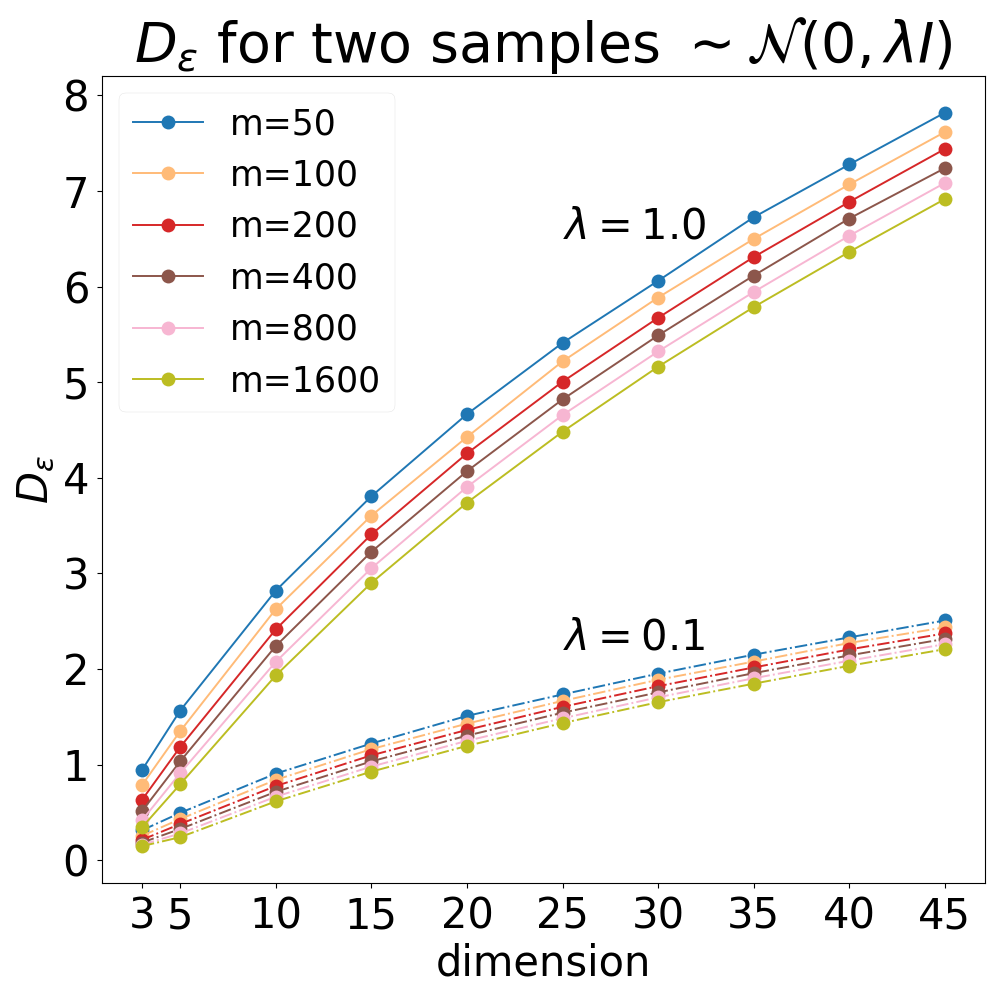
\includegraphics[width=0.8\columnwidth]{numerical-fs/plots/figures-EnKF-zeros_cov=0.1_cov=1.0.png}
\caption{Average $D_{\varepsilon}(\alpha_m^d, \beta_m^d)$ (over $20$ realizations) where $\alpha_m^d, \beta_m^d$ are two different sampling distributions with the same sample size $m$ for the same underlying $d$-dimensional Gaussian $\mathcal N(0_d, \lambda I_d)$}
\label{fig:plot-zeros--numerical-fs}
\end{figure}
In order to understand the convergence to $0$ of the above quantity [see~\eqref{eq-stablaw--numerical-fs}], we first discuss how close to zero $D_\varepsilon$ can approach numerically. In figure~\ref{fig:plot-zeros--numerical-fs} we see the average $D_\varepsilon(\alpha^d_m, \beta^d_m)$ where $\alpha_m^d=\frac{1}{m}\sum_{i=1}^m\delta_{x^{m,d}_i}$ and $\beta_m^d=\frac{1}{m}\sum_{i=1}^m\delta_{y^{m,d}_i}$, with $\{x^{m,d}_i\}$ and $\{y^{m,d}_i\}$ both samples from the same underlying $d$-dimensional Gaussian distribution $\mathcal N_d^\lambda:=\mathcal N(0_d, \lambda I_d)$. 
For `small' $\lambda$, we can expect $D_\varepsilon$ to behave in a similar fashion as if $\mathcal N_d^\lambda$ were supported on a compact set. With that in mind, we relate the numerical results shown in figure~\ref{fig:plot-zeros--numerical-fs} to the results~\ref{lem-prop--numerical-fs}--\ref{thm-zero--numerical-fs} in the appendix~\ref{sec-app--numerical-fs} by noting the following key points:

% By the phrase \textit{zero of the Sinkhorn algorithm} we mean the value of $D_\varepsilon$ obtained by using algorithm~\ref{algo-sink--numerical-fs} when the inputs are two different sampling distributions coming from the same underlying probability distribution.

\subsubsection{Drop with increase in sample size} Theorem~\ref{thm-zero--numerical-fs} explains the monotone drop in average $D_\varepsilon$ for a fixed dimension while increasing the sample size.

\subsubsection{Rise with increase in dimension} As the dimension increases, larger sample sizes are required to accurately estimate $\mathcal N_d^\lambda$. Consequently, $D_\varepsilon(\alpha_m^d, \beta_m^d)$ grows with $d$ for fixed $m$ since $\alpha_m^d, \beta_m^d$ become poorer estimators of $\mathcal N_d^\lambda$ as $d$ increases. 

 % PF 12 plots 
\begin{figure*}[!t]
\centering
\begin{subfigure}{0.3\textwidth}
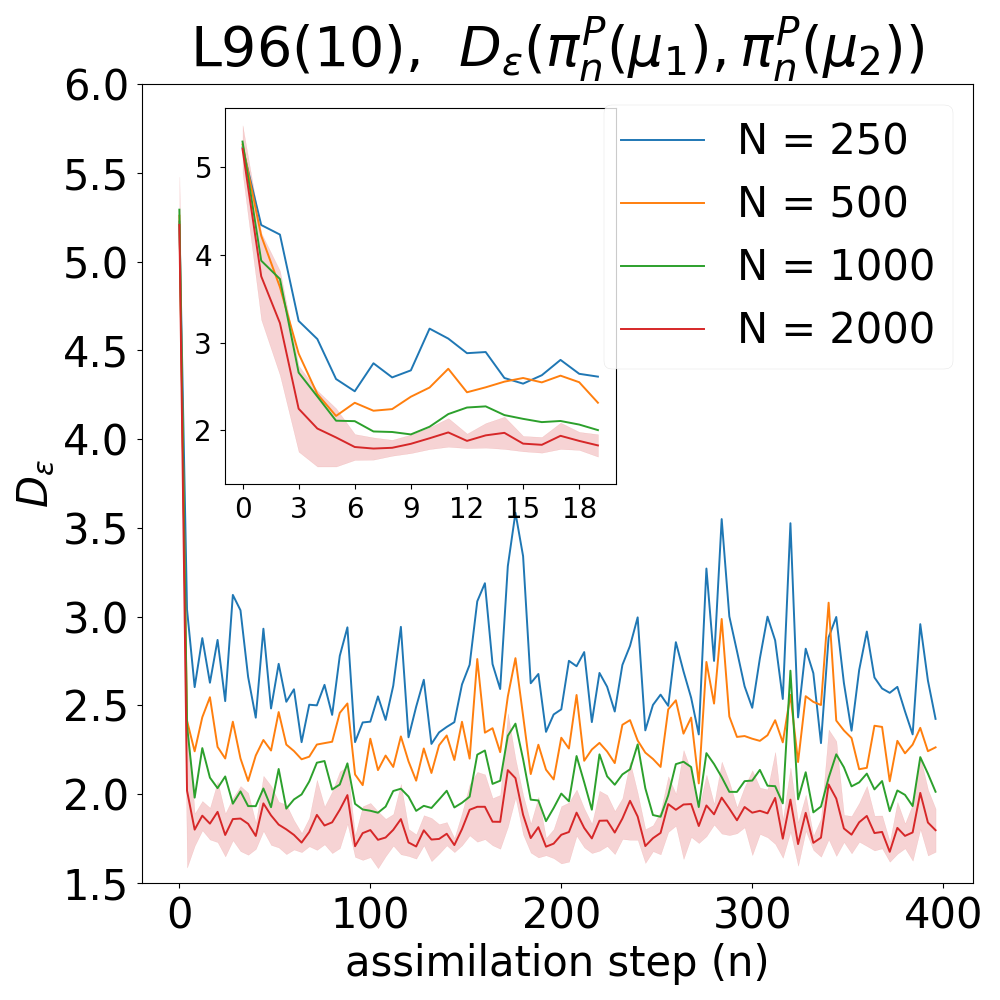
\includegraphics[width=\columnwidth]{numerical-fs/plots/figures-BPF-L96_10-1-dist_1_vs_2.png}
%\caption{dist 1 vs 2}
\end{subfigure}\hspace{0mm}%
\begin{subfigure}{0.3\textwidth}
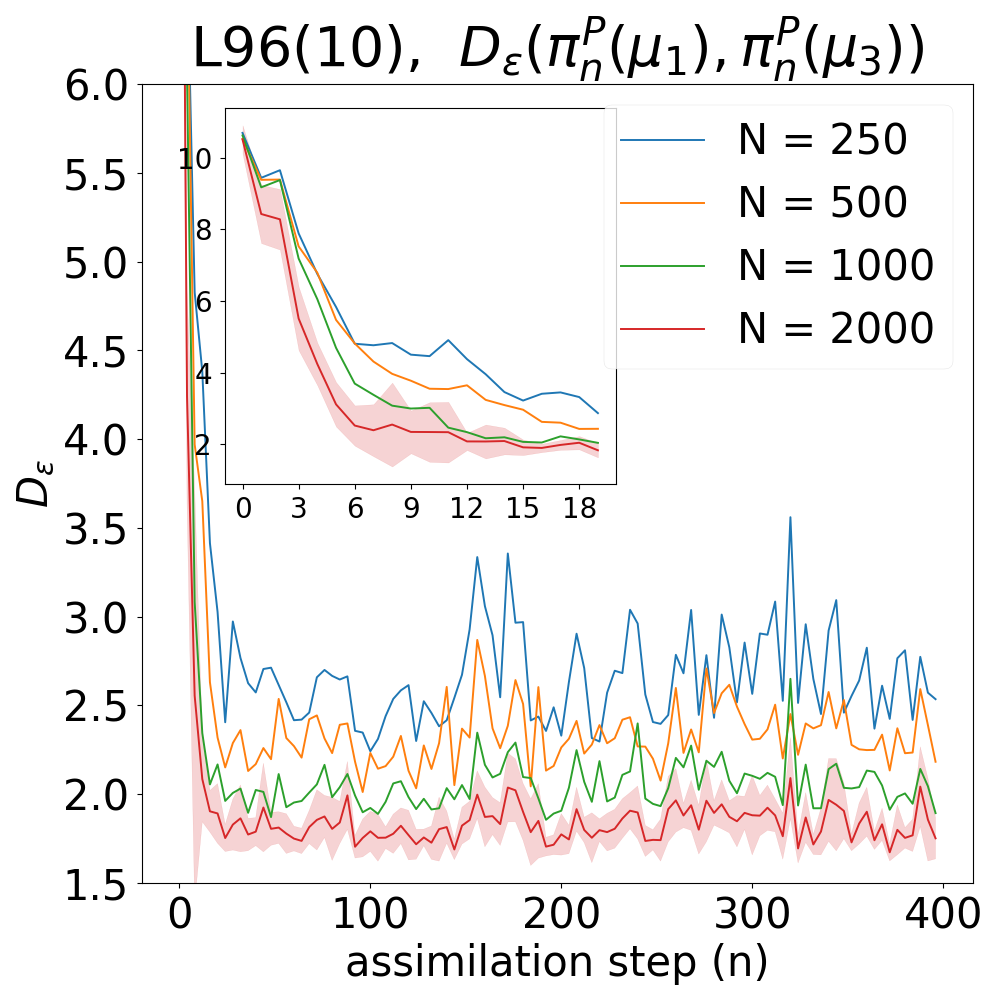
\includegraphics[width=\columnwidth]{numerical-fs/plots/figures-BPF-L96_10-1-dist_1_vs_3.png}
%\caption{dist 1 vs 3}
\end{subfigure}\hspace{0mm}%
\begin{subfigure}{0.3\textwidth}
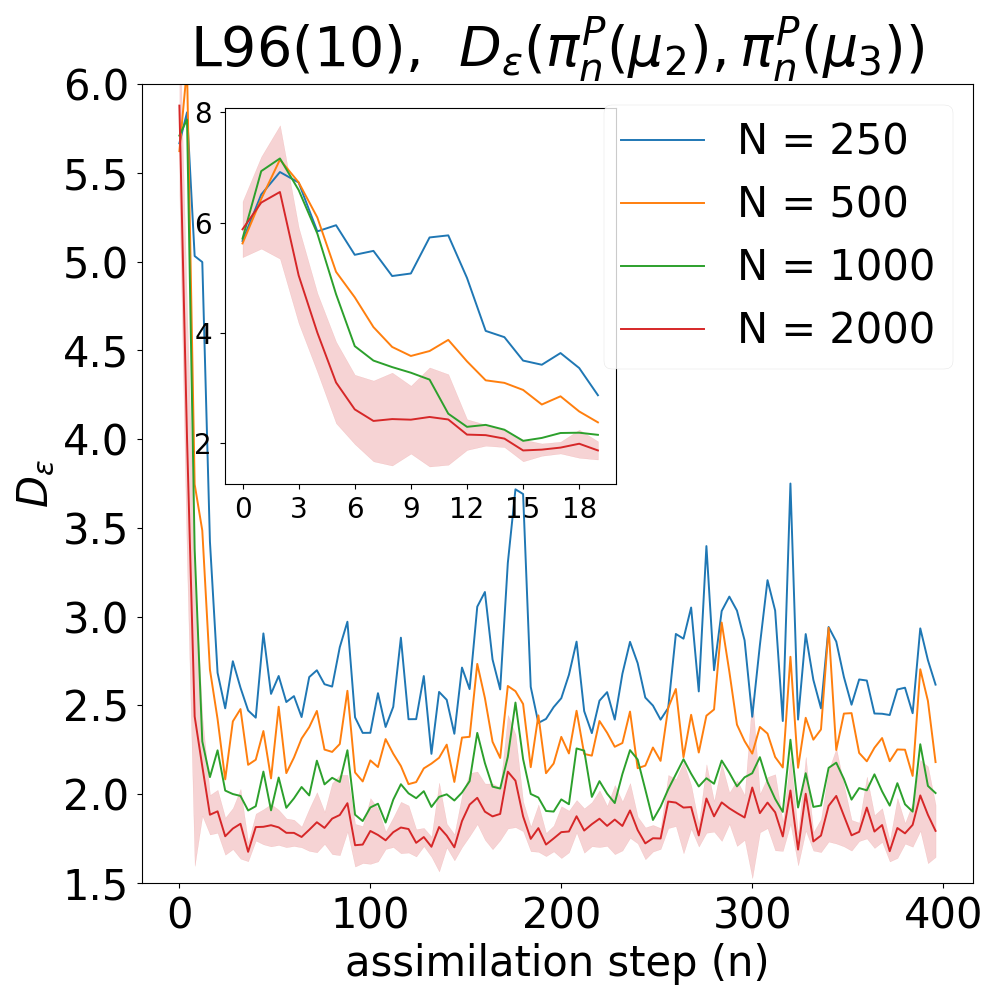
\includegraphics[width=\columnwidth]{numerical-fs/plots/figures-BPF-L96_10-1-dist_2_vs_3.png}
%\caption{dist 2 vs 3}
\end{subfigure}\hspace{0mm}%

\begin{subfigure}{0.3\textwidth}
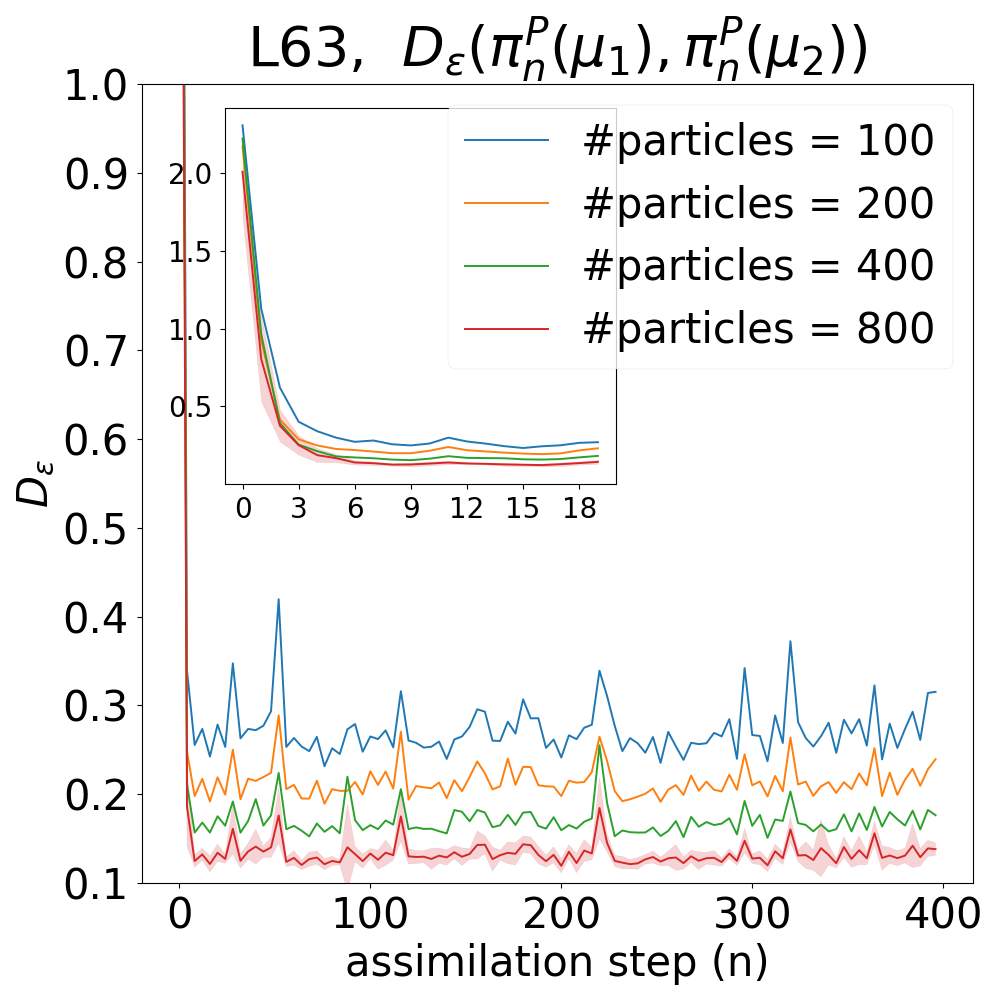
\includegraphics[width=\columnwidth]{numerical-fs/plots/figures-BPF-L63-1-dist_1_vs_2.png}
%\caption{dist 1 vs 2}
\end{subfigure}\hspace{0mm}%
\begin{subfigure}{0.3\textwidth}
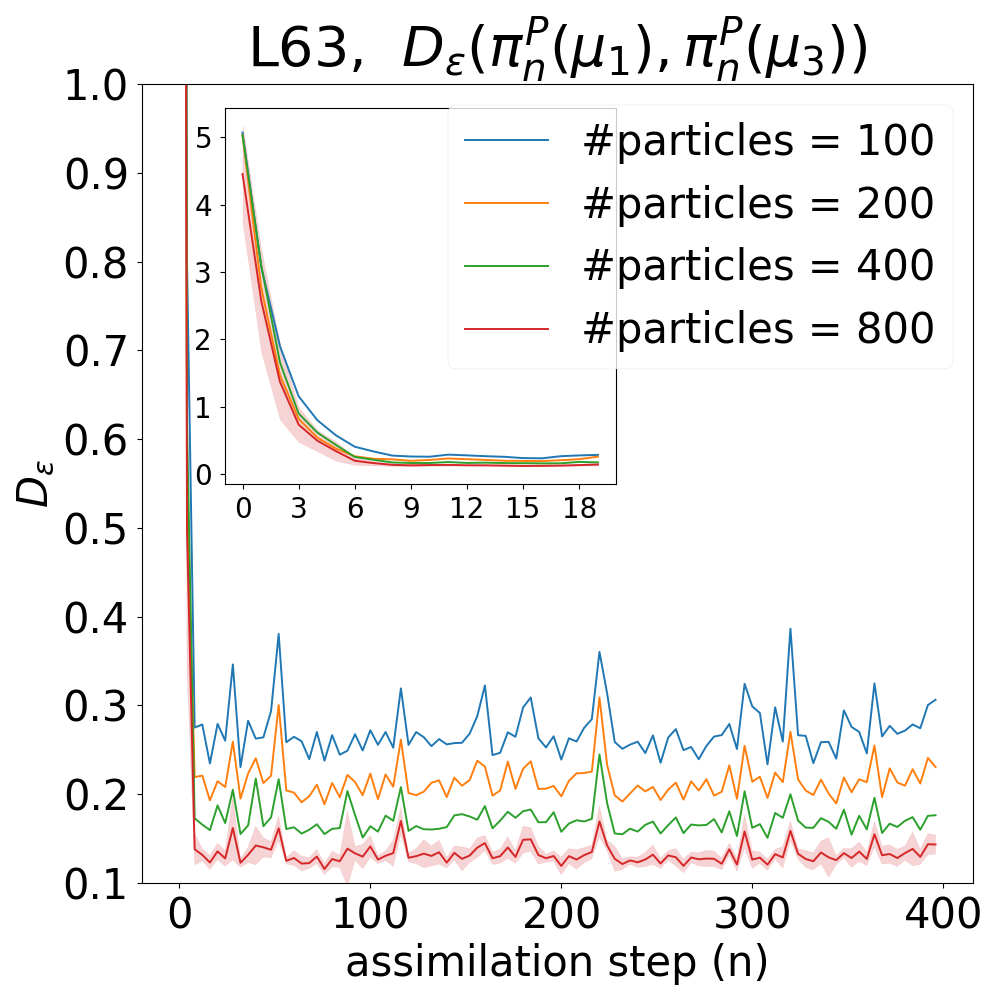
\includegraphics[width=\columnwidth]{numerical-fs/plots/figures-BPF-L63-1-dist_1_vs_3.png}
%\caption{dist 1 vs 3}
\end{subfigure}\hspace{0mm}%
\begin{subfigure}{0.3\textwidth}
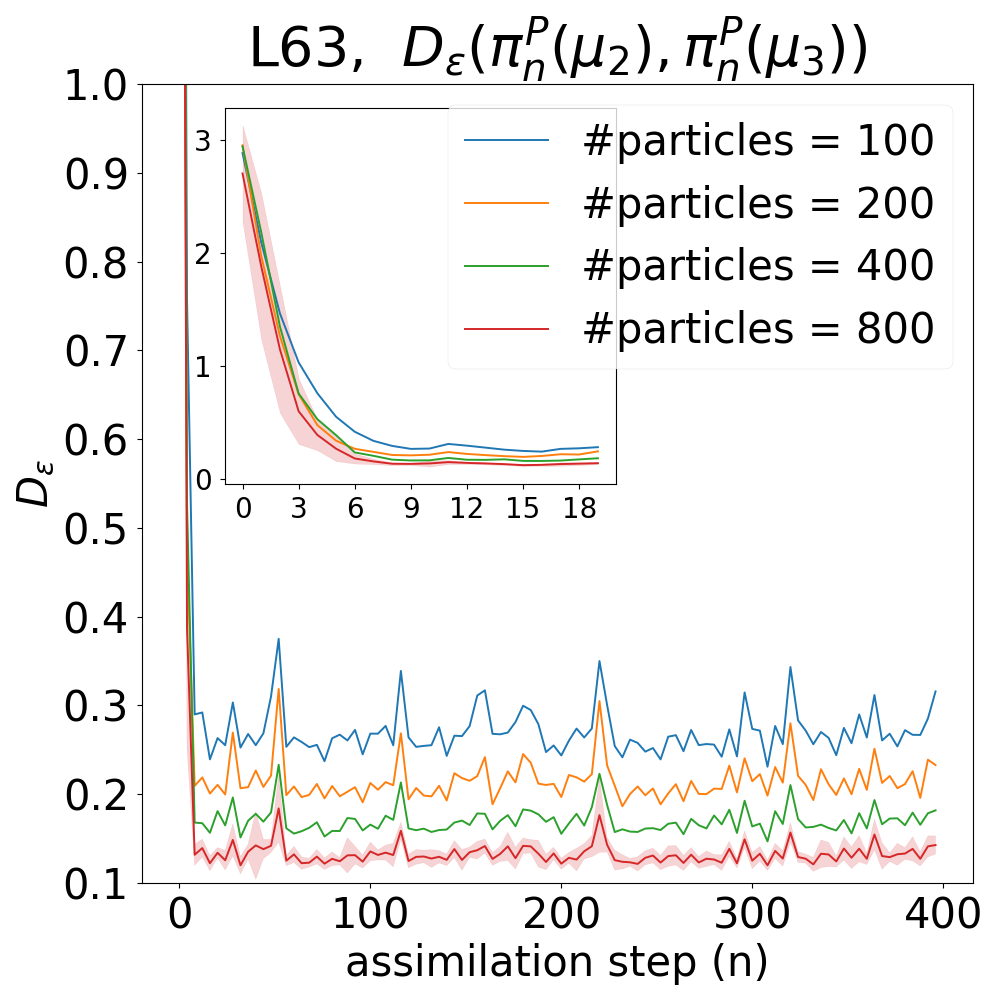
\includegraphics[width=\columnwidth]{numerical-fs/plots/figures-BPF-L63-1-dist_2_vs_3.png}
%\caption{dist 2 vs 3}
\end{subfigure}\hspace{0mm}
\caption{$D_\varepsilon$ (averaged over $10$ observation realizations) for BPF for $10$-dimensional $L96$ (row 1) and $L63$ (row 2) systems with observation covariance $\sigma^2=0.1$, for pairs of initial distributions in~\eqref{eq-3ic--numerical-fs}, with varying sample size. The line for $N = 2000$ has a band showing one standard deviation. The inset shows the drop in average $D_\varepsilon$ during the first few assimilation steps.}
\label{fig:plot-BPF--numerical-fs}
\end{figure*}

\subsubsection{Drop with decrease in covariance} Decreasing the covariance $\lambda$ has the opposite effect since, for fixed dimension $d$ and sample size $m$, smaller covariance leads to a better estimation of the underlying distribution, i.e., $\alpha_m^d, \beta_m^d$ become better estimators of $\mathcal N_d^\lambda$ as $\lambda$ decreases.

\subsubsection{Support of our distributions} Since the true trajectories for both systems (L63, L96) lie on bounded attractors, we can assume that true filtering distributions are supported on a compact set. Consequently, in the filtering experiments shown later, the zero of the Sinkhorn algorithm shows qualitatively similar behavior (e.g., in figure~\ref{fig:plot-BPF--numerical-fs}) with respect to dimension as seen in figure~\ref{fig:plot-zeros--numerical-fs}.

\subsection{Particle Filter}
Here we use the notation $\pi^{P, N}_n$ for $\hat\pi_n$ obtained by alogithm~\ref{algo-bpf--numerical-fs} with $N$ particles (omitting $N$ for brevity when value of $N$ is clear from context). Figure~\ref{fig:plot-BPF--numerical-fs} shows $\mathbb E[D_\varepsilon(\hat\pi_n(\mu_i), \hat\pi_n(\mu_j))], \ i \ne j$ as a function of $n$. We note some important conclusions.
\subsubsection{BPF quickly forgets the initial distribution} From the insets in figure~\ref{fig:plot-BPF--numerical-fs} we can see that for every pair $(\mu_i, \mu_j)$ of initial distributions, $\mathbb E\left[D_\varepsilon(\pi^P_n(\mu_i), \pi^P_n(\mu_j))\right]$ stabilizes in the first few assimilation steps. In fact, this behavior is consistent with exponential stability of particle filters \cite{chigansky2009intrinsic}.
\subsubsection{Dependence on the number of particles} 
$\mathbb E\left[D_\varepsilon(\pi^{P, N}_n(\mu_i), \pi^{P, N}_n(\mu_j))\right]$ for a fixed $n$ decreases monotonically with increasing $N$ for both L63 and L96 and for both observation covariances for all pairs $i\neq j$.
%$\pi^{P,N}_n$ weak$^*$ converges to the true filtering distribution $\pi_n$ as $N\to\infty$ \cite{van2008hidden}. This fact along with theorem \ref{thm-zero--numerical-fs} is enough for explaining the drop in $D_\varepsilon$ in figure~\ref{fig:plot-BPF--numerical-fs} for fixed $n$ as we increase $N$.
\subsubsection{Stability}
Suppose the best possible filtering distribution that can be computed by the particle filter is $\pi^{P,*}_n=\lim_{N\to\infty}\pi^{P,N}_n$. Figure~\ref{fig:plot-BPF--numerical-fs} is consistent with the condition
\begin{align*}
    \lim_{n\to\infty}\liminf_{N\to\infty}\mathbb E[D_\varepsilon(\pi^{P,N}_n(\mu_i), \pi^{P,N}_n(\mu_j))]=0\;\forall\; i\neq j
\end{align*}
since fixing $n$ and increasing $N$ results in a steady drop in $D_\varepsilon$ averaged over observation realizations. By theorem \ref{thm-stable--numerical-fs} this condition is sufficient for concluding
\begin{align*}
    \lim_{n\to\infty}\mathbb E[D_\varepsilon(\pi^{P,*}_n(\mu_i), \pi^{P,*}_n(\mu_j))]=0\;\forall\; i\neq j
\end{align*}
\subsubsection{Dependence on observation covariance} All plots in figure~\ref{fig:plot-BPF--numerical-fs} correspond to observation covariance $\sigma^2=0.1$. The other case $\sigma^2=1.0$ mentioned in \ref{ssec-models--numerical-fs} results in plots that are qualitatively similar to the ones in figure~\ref{fig:plot-BPF--numerical-fs} and we omit those plots here. In our experiments, stability of particle filter was not seen to be affected by observation covariance. 

\subsection{EnKF}
% Enkf 3 plot, 1 is left:
\begin{figure*}[!t]
\centering
\begin{subfigure}{.3\textwidth}
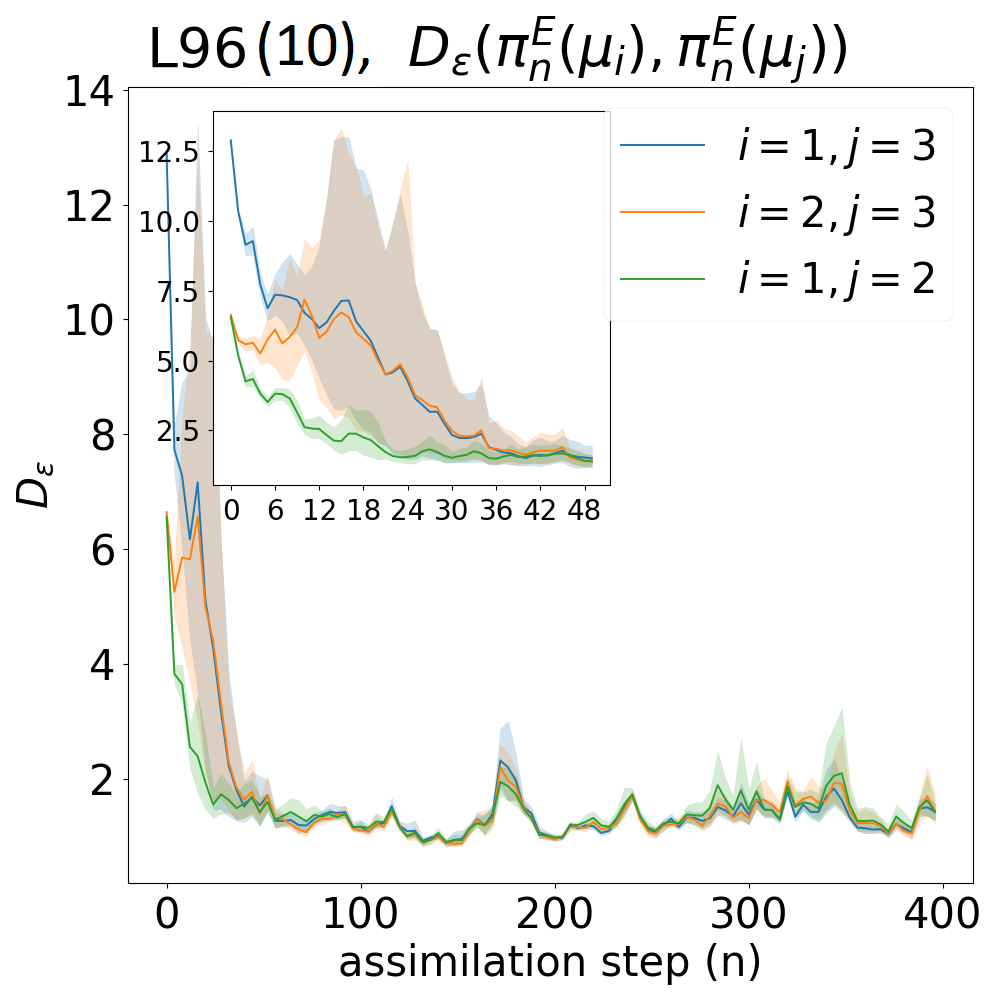
\includegraphics[width=\columnwidth]{numerical-fs/plots/figures-EnKF-stable_50_L96_10dim.png}%
%\caption{N=50 with localization}%
%\label{sub@fig:plot-enkf50--numerical-fs}%
\end{subfigure}\hspace{0mm}% 
\begin{subfigure}{.3\textwidth}
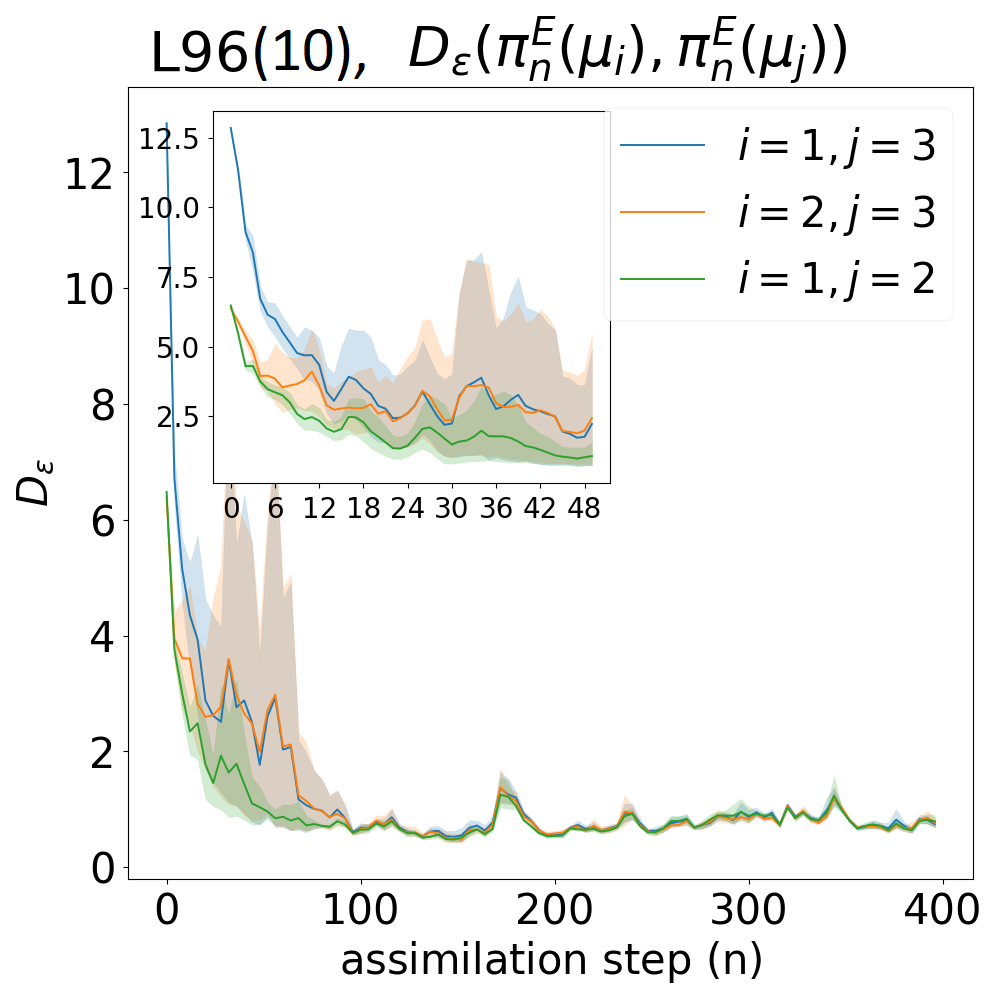
\includegraphics[width=\columnwidth]{numerical-fs/plots/figures-EnKF-stable_200_L96_10dim.png}%
%\caption{N=200 without localization}%
%\label{sub@fig:plot-enkf200--numerical-fs}%
\end{subfigure}\hspace{0mm}%
\begin{subfigure}{.3\textwidth}
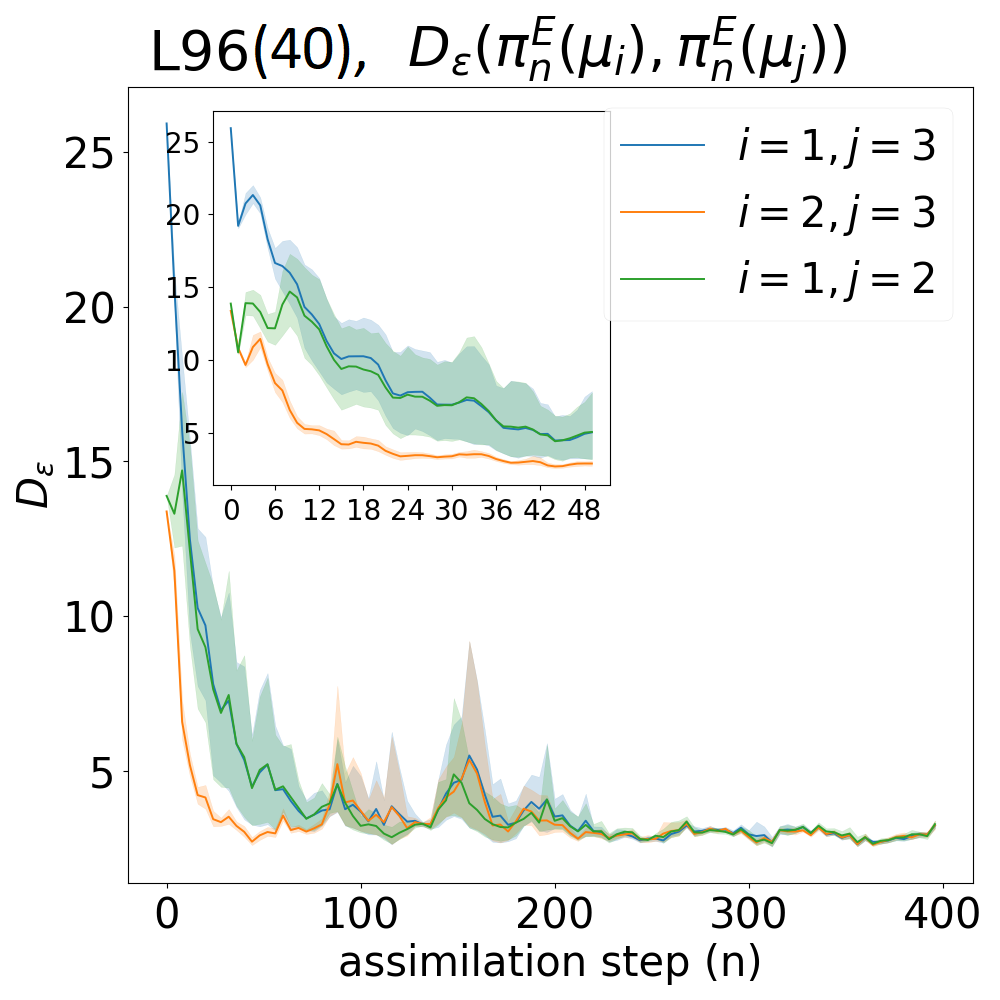
\includegraphics[width=\columnwidth]{numerical-fs/plots/figures-EnKF-stable_50_loc_L96_40dim.png}%
%\caption{$D_\varepsilon$ for $\mu_{i}$ with N=50,200}%
%\label{sub@fig:plot-enkfL96-40--numerical-fs}%
\end{subfigure}%
\caption{$D_\varepsilon$ (averaged over $10$ observation realizations, with one standard deviation confidence band) for EnKF for $10$-dimensional L96 with $N=50$ with localization (left), $N=200$ without localization (middle) for observation covariance $\sigma^2=0.1$, and for $40$-dimensional L96 with $N=50$ with localization (right) with observation covariance $\sigma^2=1.0$ for pairs of initial distributions in \ref{eq-3ic--numerical-fs}. The inset shows the drop in $D_\varepsilon$ for the first 50 assimilation steps.}
\label{fig:plot-enkfL96-10--numerical-fs}
\end{figure*}
Here we use the notation $\pi^{E,N}_n$ for $\hat\pi_n$ obtained by alogithm~\ref{algo-enkf--numerical-fs} with ensemble size $N$. We might omit $N$ for brevity.
\subsubsection{Drop in $D_\varepsilon$ over time}
From figure~\ref{fig:plot-enkfL96-10--numerical-fs}, we see that for every pair $(\mu_i, \mu_j)$ of initial distributions $D_\varepsilon(\pi^E_n(\mu_i), \pi^E_n(\mu_j))$ decreases with time rapidly within the first $50$ assimilation steps and beyond $100$ assimilation steps, the observation average of $D_\varepsilon$ for filters with different pairs initial distributions are similar and have very little variance.
\subsubsection{Variation with respect to observation realization} We see that the variation of $D_\varepsilon$ for different observation realizations (shown by the shaded bands in left two panels in figure~\ref{fig:plot-enkfL96-10--numerical-fs} and in top row in figure~\ref{fig:plot-BPF--numerical-fs}) is larger for the case of EnKF when compared to the particle filter for initial times (e.g. $n < 100$ for the 10-dimensional L96 model). On the other hand, for larger times (approx.~$n > 100$), the variation for EnKF is significantly smaller than the particle filter.
% \subsubsection{}
% For $10$-dimensional L96 system, we see that the $D_\varepsilon$ between the filer with localization and without localization for the same initial distribution are different but stable.  
\subsubsection{Effect of localization}
EnKF with small ensemble size needs localization which, however, is an ad-hoc procedure to prevent filter divergence and may not approximate the true filter. Figure~\ref{fig:plot-enkfL96-10--numerical-fs} for $10$-dimensional L96 (left panel) and for $40$-dimensional L96 (right panel) shows that for $N=50$ with localization length 4, the EnKF is stable, whereas the middle panel shows the stability (with the same configuration as the left panel) for $10$-dimensional L96 without localization, but with larger ensemble size $N=200$. This indicates that that localization does not affect EnKF's stability properties.

% L96-40 dimensions plot
% \begin{figure}
% \centering
% 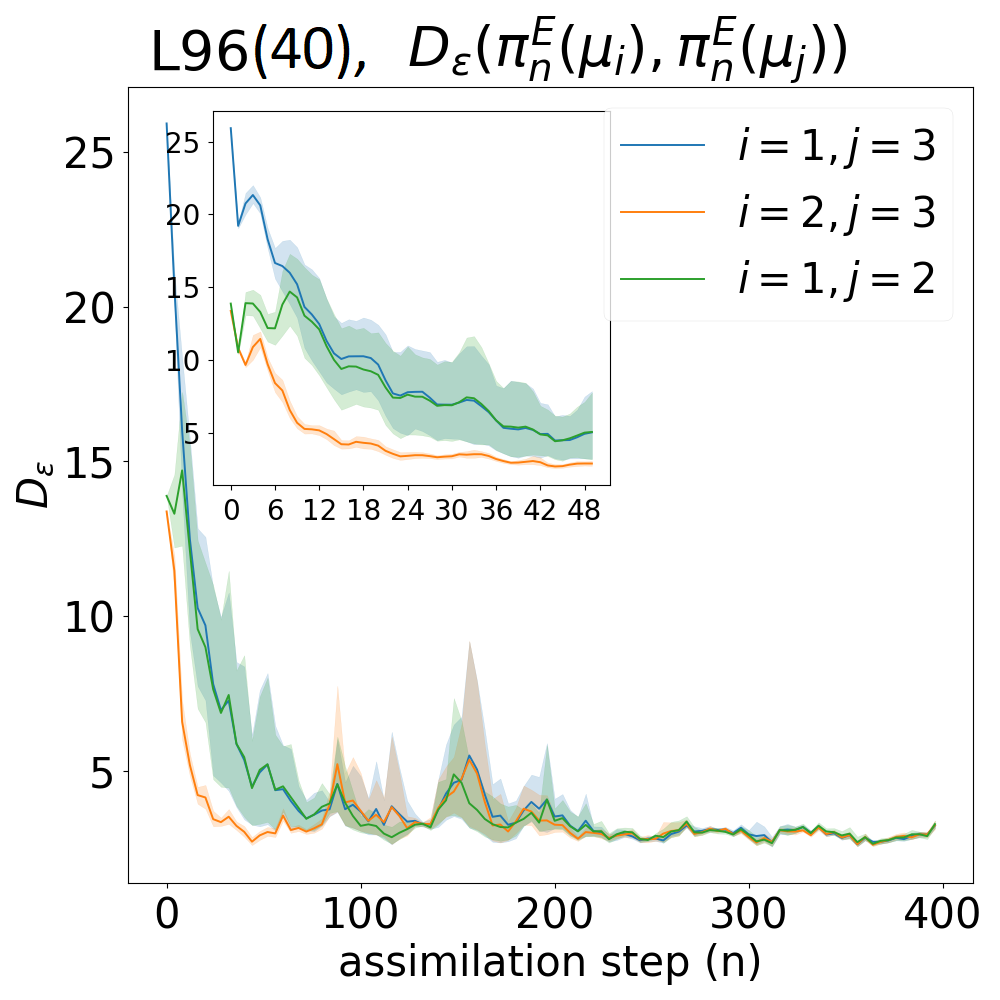
\includegraphics[width=0.8\columnwidth]{numerical-fs/plots/figures-EnKF-stable_50_loc_L96_40dim.png}
% \caption{$D_\varepsilon$ for $40$-dimensional L96 model for N=50 with localization length=4.}
% \label{fig:plot-enkfL96-40--numerical-fs}
% \end{figure}

\subsection{BPF vs EnKF}
\begin{figure}
\centering
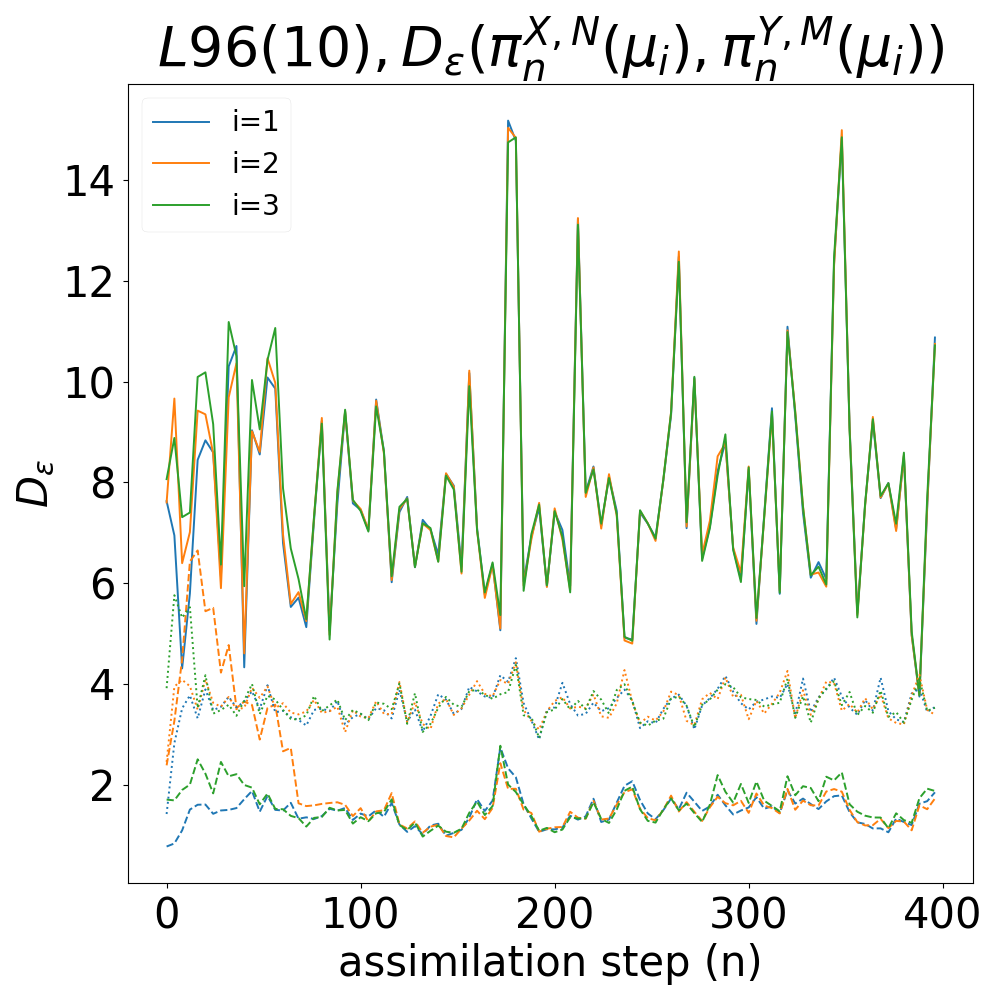
\includegraphics[width=0.8\columnwidth]{numerical-fs/plots/figures-BPF-L96_10-EnKF-distance between different filters.png}
\caption{Comparison between filters for $10$-dimensional L96 and $\sigma^2=1.0$. The solid lines on the top show average $D_\varepsilon$ between EnKF without localization with $N = 200$ and BPF with $M = 2000$. The dotted lines in the middle show average  $D_\varepsilon$ between  BPF with $N = 250$ and BPF with $M = 2000$. The dashed lines at the bottom show average  $D_\varepsilon$ between EnKF without localization with $N = 200$ and EnKF with localization with $M = 50$. In each case, different colors are for different initial conditions from~\eqref{eq-3ic--numerical-fs}.} 
\label{fig:plot-compare--numerical-fs}
\end{figure}
We now compare the BPF and EnKF for the case of $10$-dimensional L96 with $\sigma^2=1.0$ with the same true trajectory and observation realizations. This is shown in figure~\ref{fig:plot-compare--numerical-fs}. {In the following discussion we assume BPF with 2000 particles to be a decent approximation for the true filter and refer to them interchangably.} We note a few important points.
\subsubsection{Poor approximation of the true filter by EnKF} The three lines towards the top show the distance between EnKF and BPF, for three different initial conditions. We see that EnKF produces distributions that are significantly different from the true filter, for all the initial distributions. But recall that for this setup, the EnKF is stable (as is the BPF too), i.e., the distance between EnKF with different initial conditions is smaller (as seen in figures~\ref{fig:plot-BPF--numerical-fs}-\ref{fig:plot-enkfL96-10--numerical-fs}) than the distance between the BPF and EnKF
\subsubsection{BPF is closer to the true filter than is EnKF} The three lines in the middle show the distance between BPF with $N=250$ and $N=2000$ (putatively true filter). We see that in comparison with EnKF with $N=200$ particles, BPF with similar ensemble size (250 particles) is much closer to the true filter.
\subsubsection{EnKF with different ensemble size are very similar} The bottom three lines in figure~\ref{fig:plot-compare--numerical-fs} show $D_\varepsilon$ between EnKF with different ensemble size, which shows that the EnKF is quite stable with respect to changes in the ensemble size, even though it is not very close to the true filter -- thus EnKF is stable but biased, whereas BPF is stable and unbiased. A more detailed study of the reasons for this behaviour will be taken up in the future.

% %trial and all error : this is to be removed.
% \begin{figure*}
% \centering
% %\begin{tabular}{ccc}
% \subcaptionbox{caption\label{1--numerical-fs}}{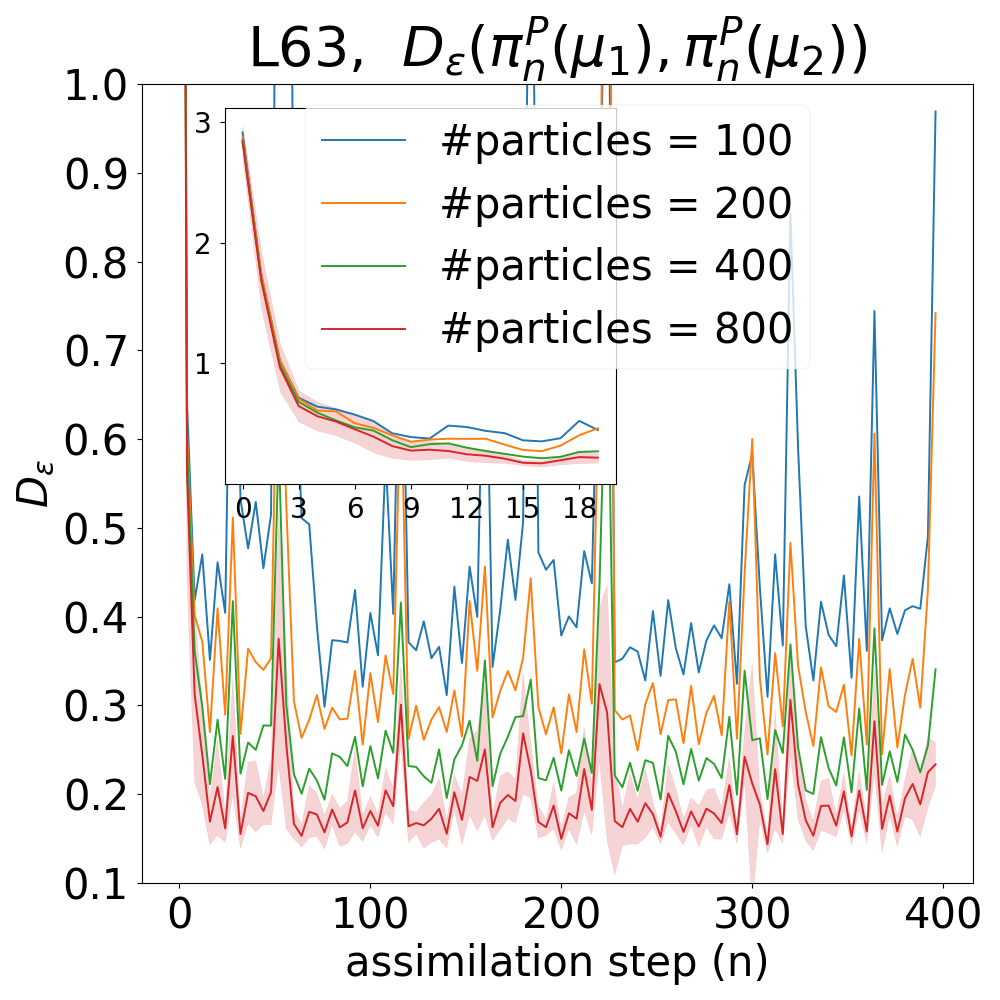
\includegraphics[width=0.28\textwidth]{numerical-fs/plots/figures-BPF-L63-0-dist_1_vs_2.png}}\hspace{0mm}
% \subcaptionbox{caption\label{2--numerical-fs}}{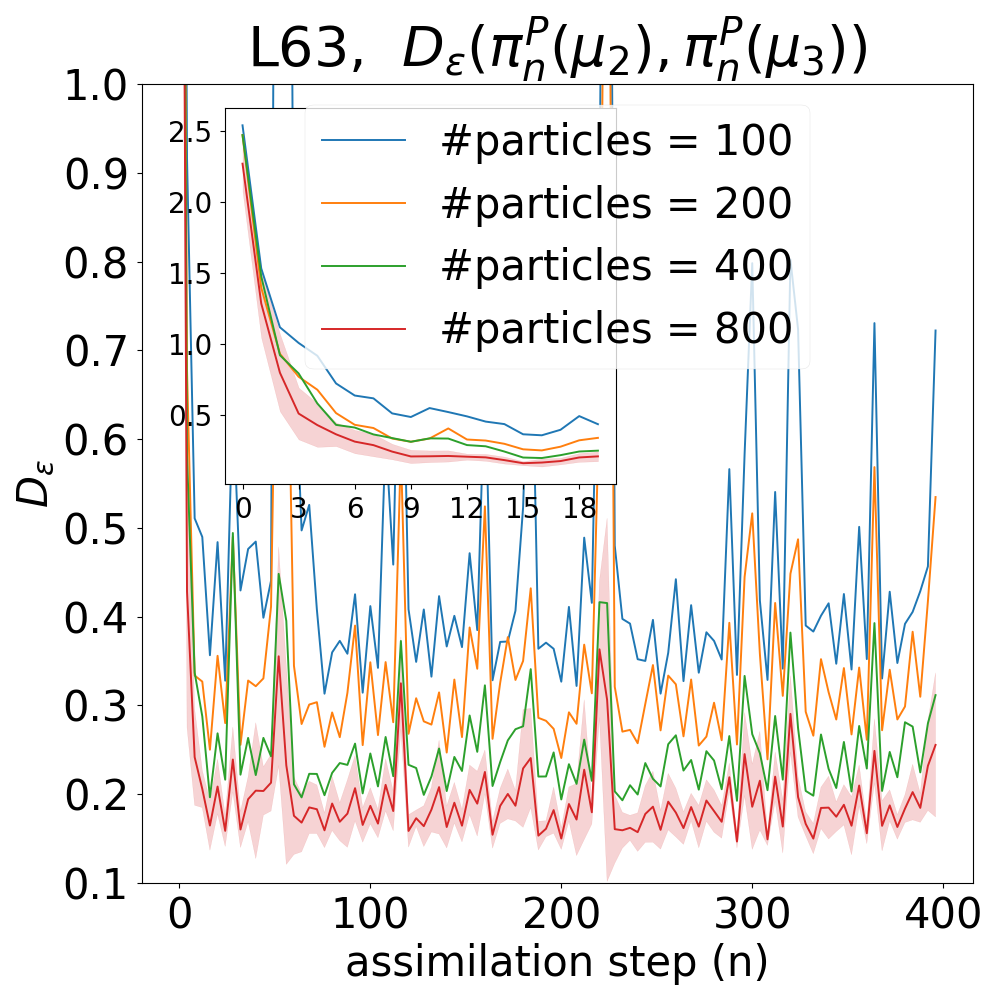
\includegraphics[width =0.28\textwidth]{numerical-fs/plots/figures-BPF-L63-0-dist_2_vs_3.png}}\hspace{0mm}
% \subcaptionbox{caption\label{2--numerical-fs}}{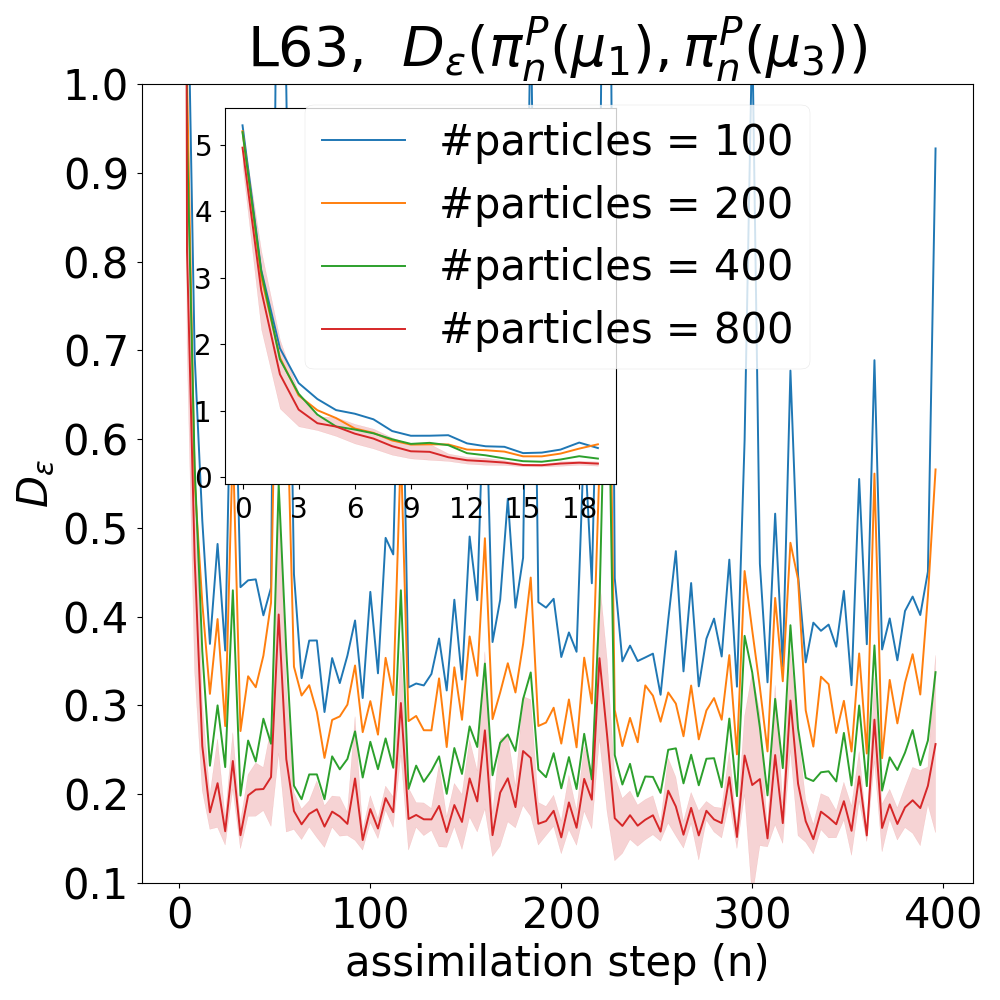
\includegraphics[width = 0.28\textwidth]{numerical-fs/plots/figures-BPF-L63-0-dist_1_vs_3.png}}\hspace{0mm}//%
% \subcaptionbox{caption\label{1--numerical-fs}}{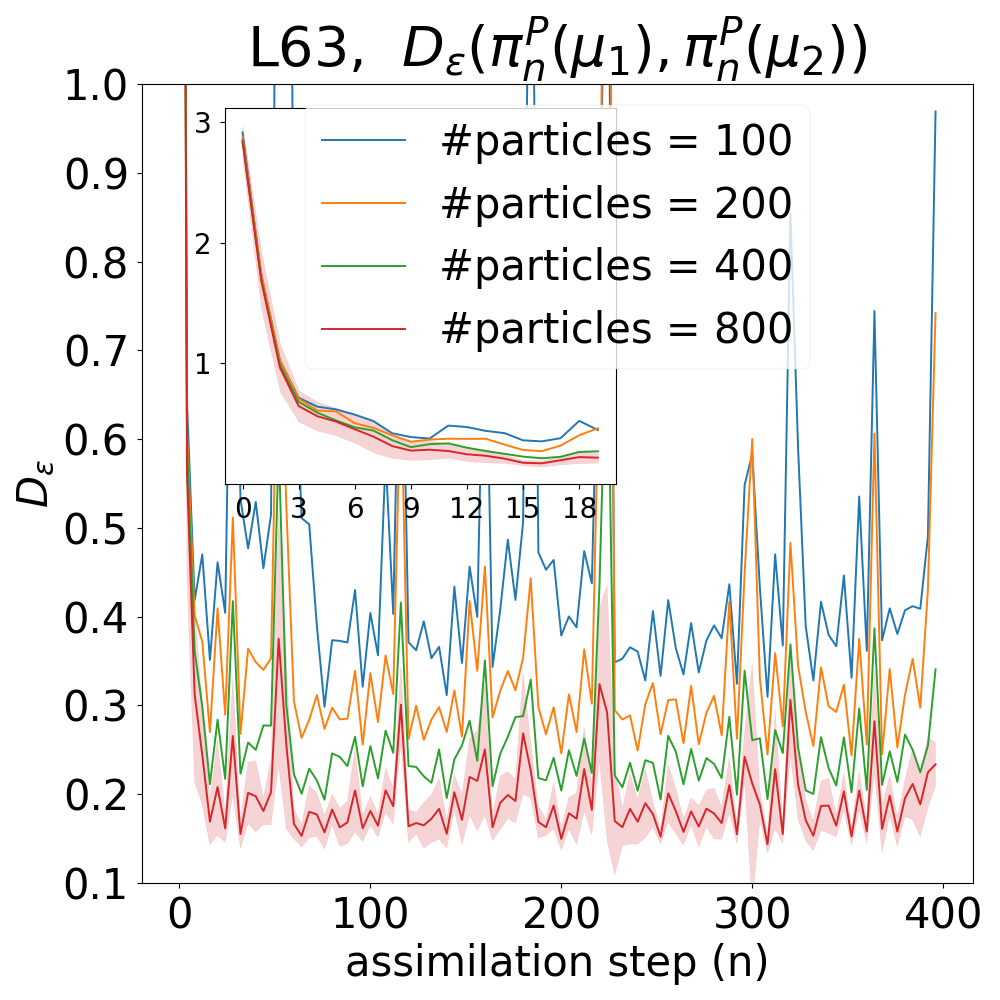
\includegraphics[width=0.28\textwidth]{numerical-fs/plots/figures-BPF-L63-0-dist_1_vs_2.png}}\hspace{0mm}
% \subcaptionbox{caption\label{2--numerical-fs}}{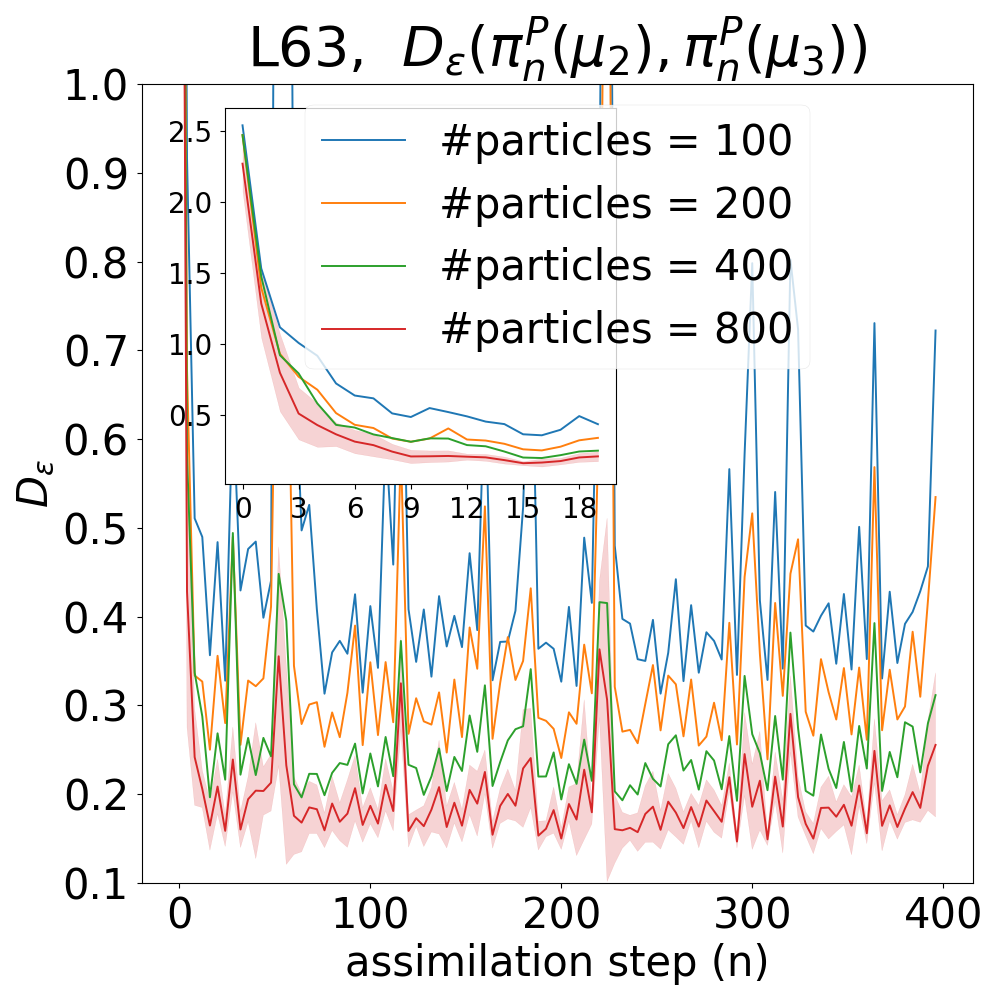
\includegraphics[width =0.28\textwidth]{numerical-fs/plots/figures-BPF-L63-0-dist_2_vs_3.png}}\hspace{0mm}
% \subcaptionbox{caption\label{2--numerical-fs}}{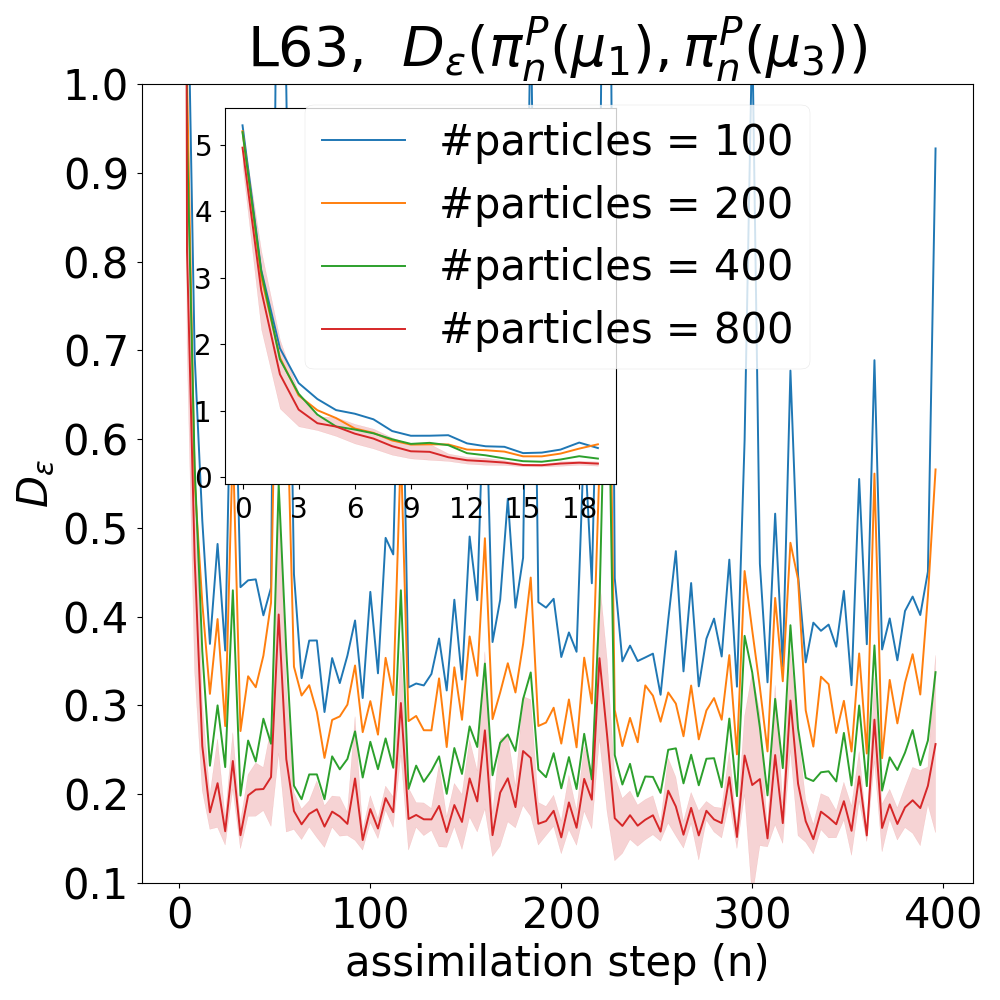
\includegraphics[width = 0.28\textwidth]{numerical-fs/plots/figures-BPF-L63-0-dist_1_vs_3.png}}\hspace{0mm}//
% %\end{tabular}
% \caption{caption}
% \label{fig2--numerical-fs}
% \end{figure*}

% \begin{figure*}[p]
% \begin{tabular}{c|c|c|c}

% {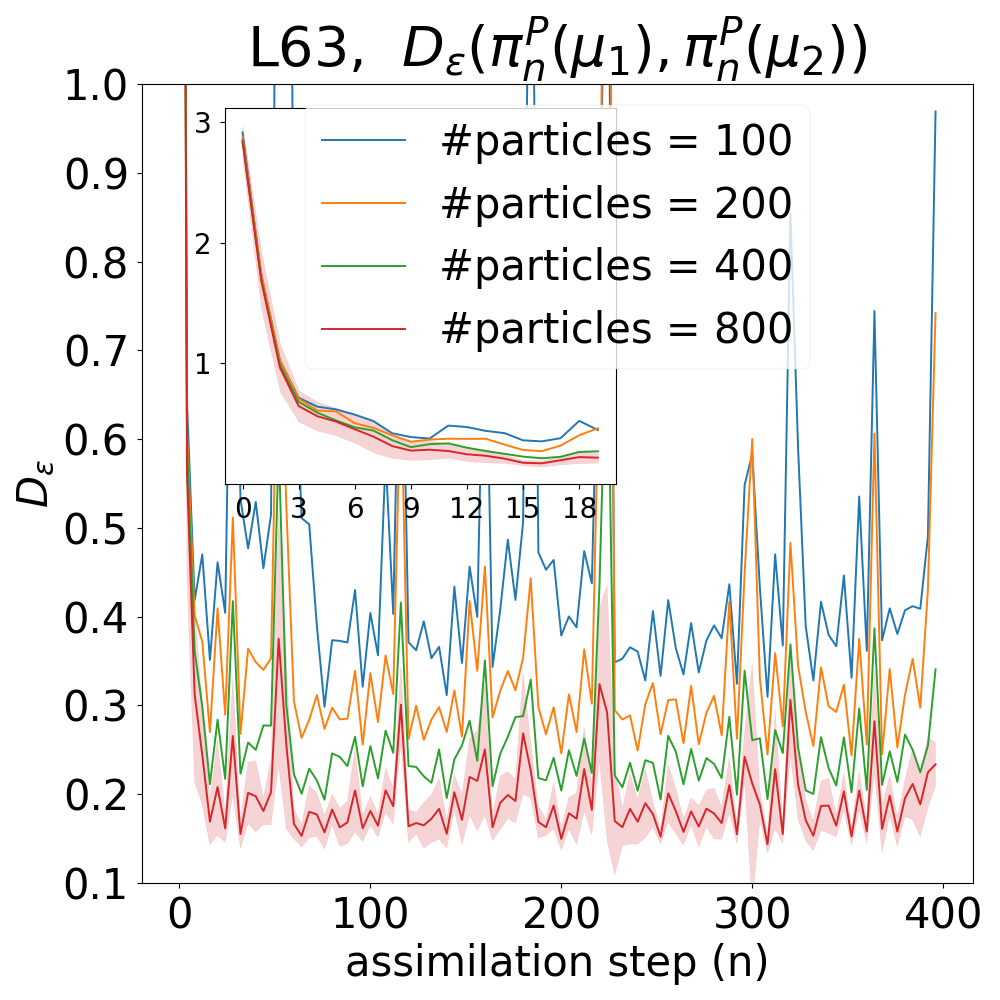
\includegraphics[width=0.2\textwidth]{numerical-fs/plots/figures-BPF-L63-0-dist_1_vs_2.png}} &
% {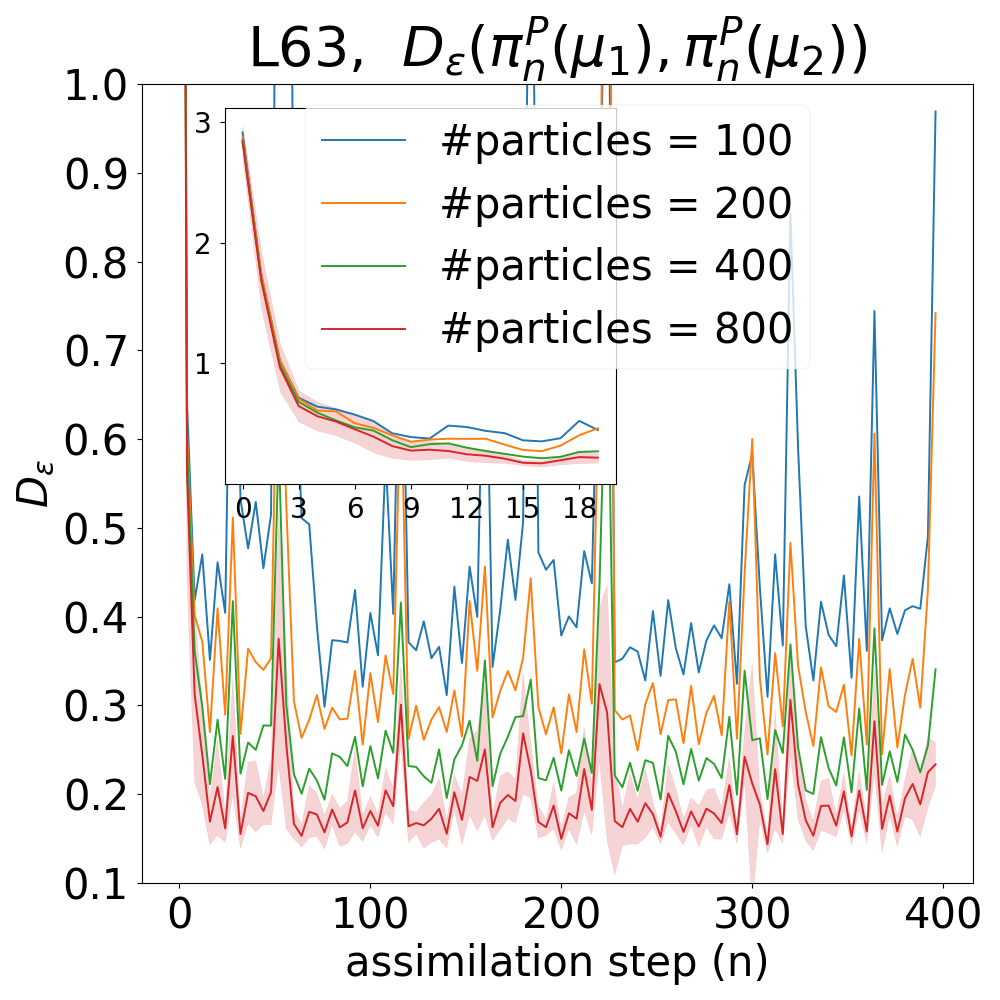
\includegraphics[width=0.2\textwidth]{numerical-fs/plots/figures-BPF-L63-0-dist_1_vs_2.png}} &
% {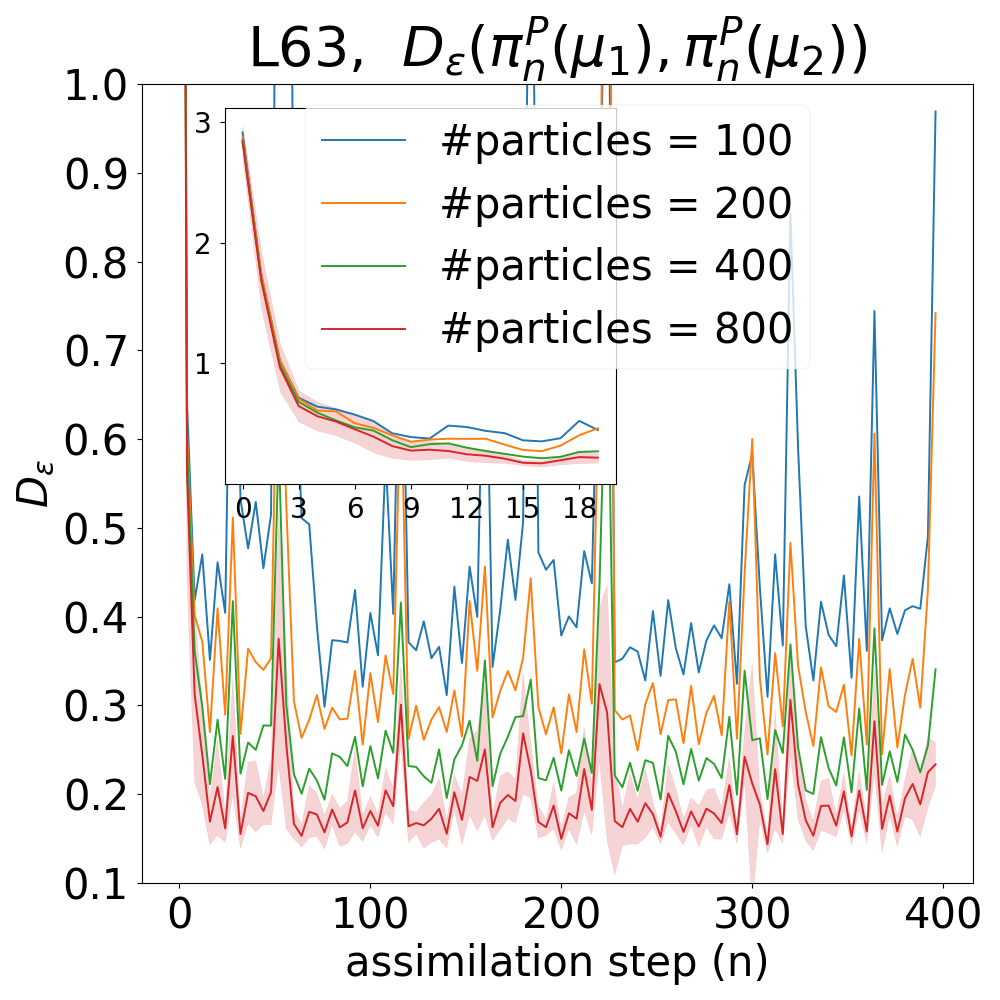
\includegraphics[width=0.2\textwidth]{numerical-fs/plots/figures-BPF-L63-0-dist_1_vs_2.png}} \\

% {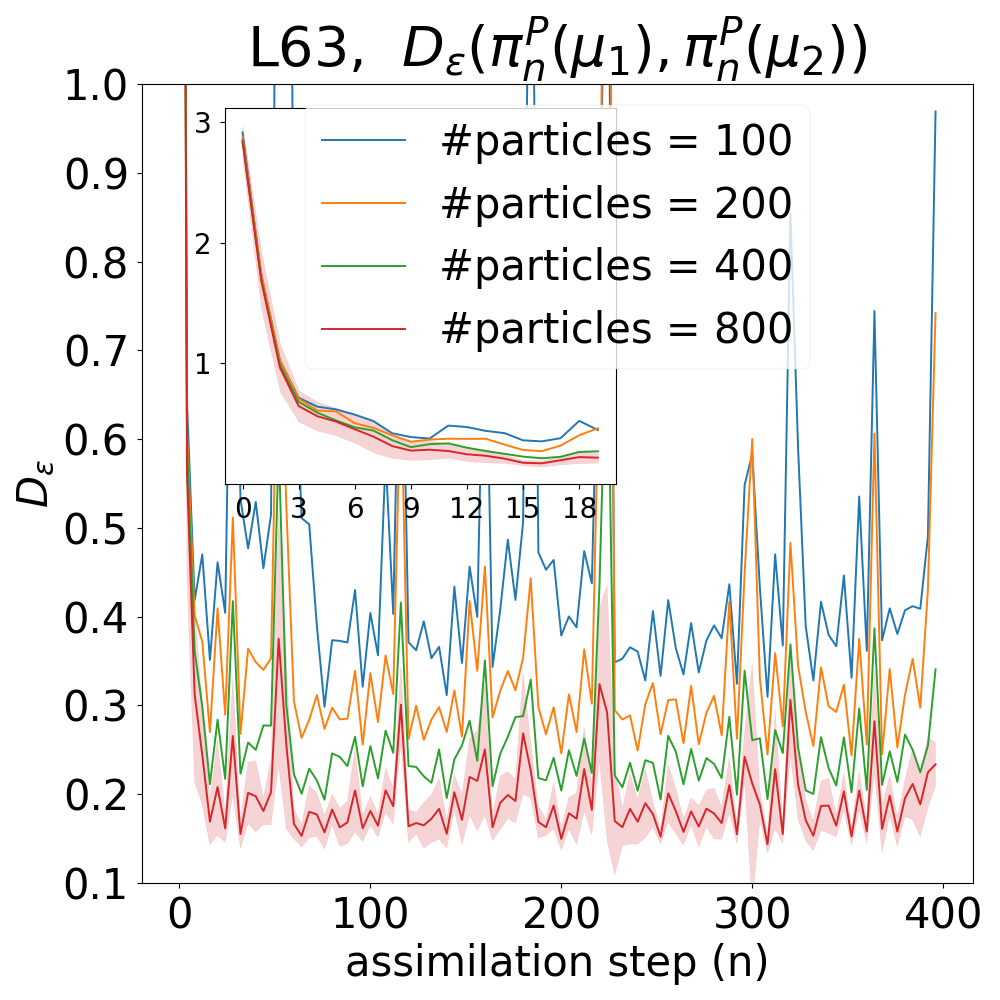
\includegraphics[width=0.2\textwidth]{numerical-fs/plots/figures-BPF-L63-0-dist_1_vs_2.png}} &
% {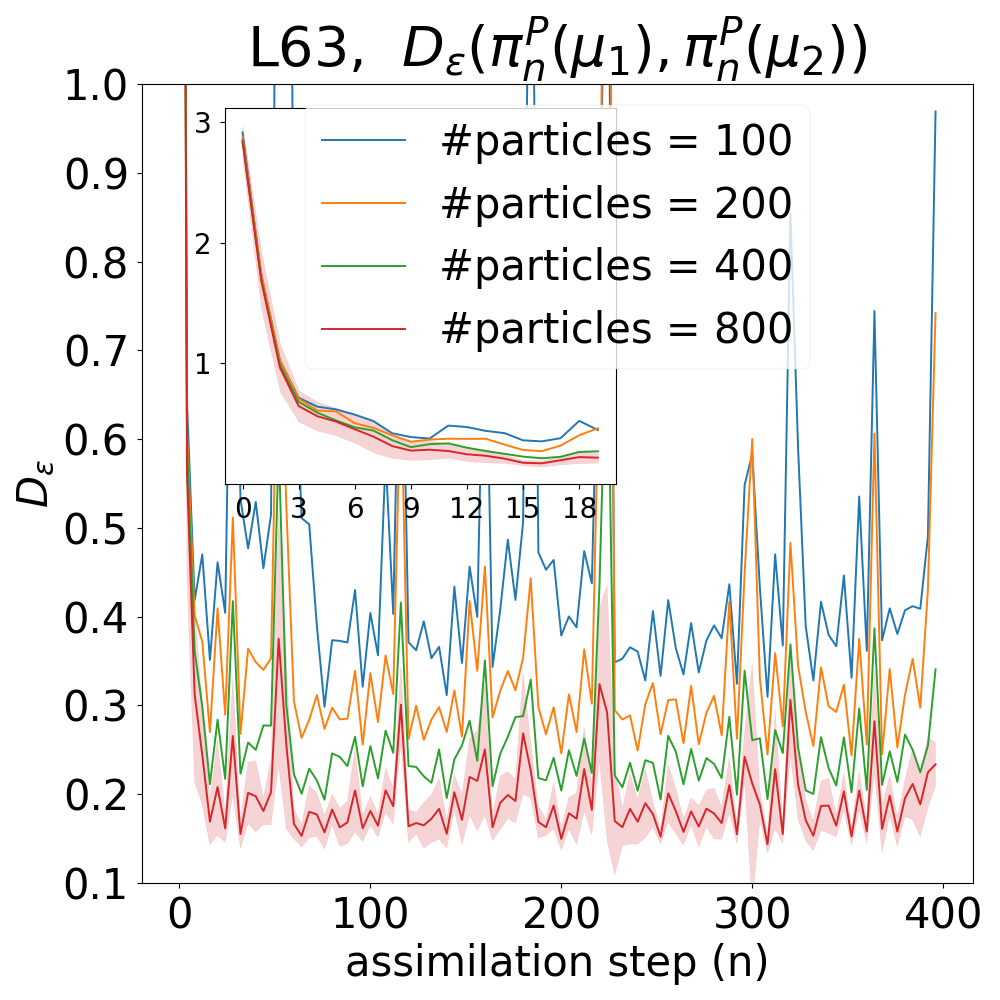
\includegraphics[width=0.2\textwidth]{numerical-fs/plots/figures-BPF-L63-0-dist_1_vs_2.png}} &
% {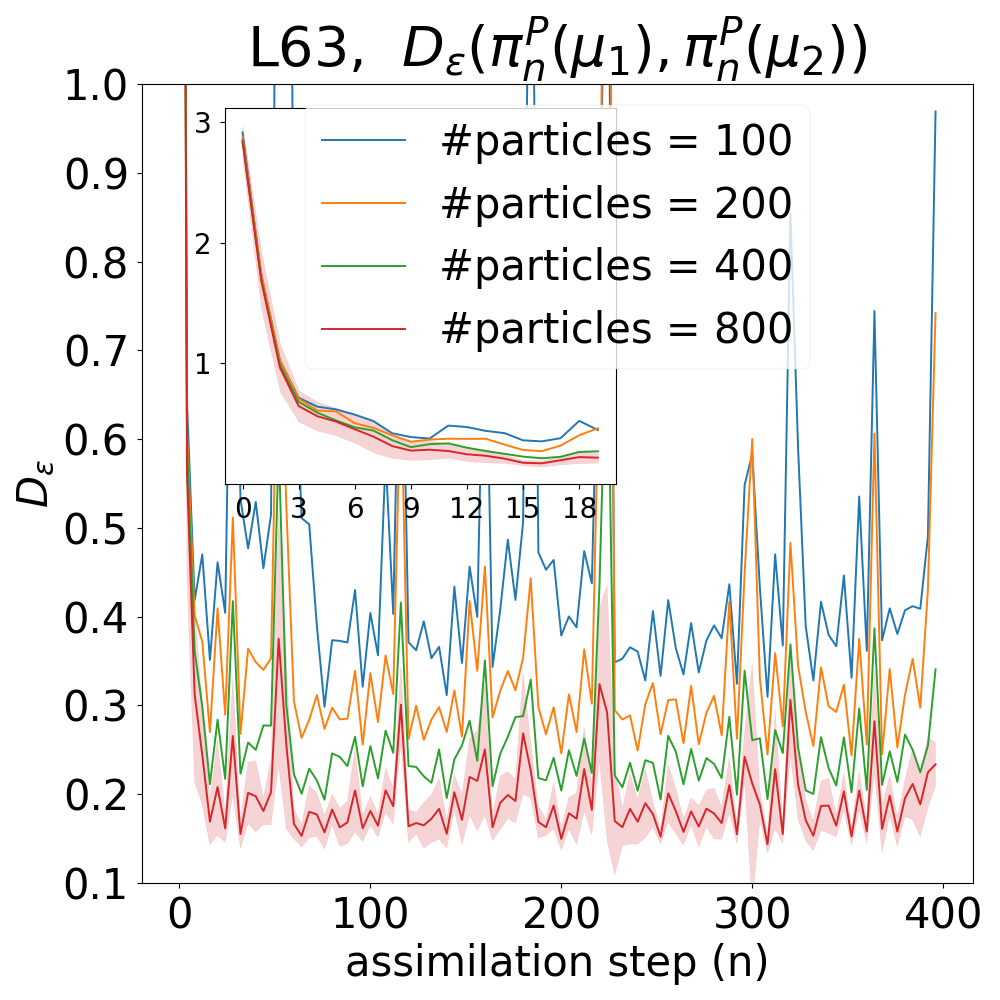
\includegraphics[width=0.2\textwidth]{numerical-fs/plots/figures-BPF-L63-0-dist_1_vs_2.png}} \\

% \end{tabular}
% \caption{Input Images}
% \end{figure*}





















%% -------------------------------------
\section{Discussion} \label{sec-disc--numerical-fs}
% \subsection{Explanation of the zero of the $S_\varepsilon$ algorithm}.
% \subsection{Explanation of the drop in $S_\varepsilon$ with increasing number of particles}

The main focus of this study was to develop a novel methodology to assess nonlinear filter stability using recently introduced techniques for calculating Wasserstein distances between distributions. We show that the particle filter and ensemble Kalman filter are stable when applied to a wide range of chaotic, deterministic dynamical systems, but the EnKF fails to capture the true filtering distribution.

We expect that the use of numerical algorithms for computing distances between the distributions will be a powerful tool for understanding nonlinear filters, leading to several avenues for further exploration. One direction of particular interest in earth sciences is to examine the relation between filter stability and the dynamical properties of the systems being observed.

%\addtolength{\textheight}{-12cm}
% This command serves to balance the column lengths
% on the last page of the document manually. It shortens
% the textheight of the last page by a suitable amount.
% This command does not take effect until the next page
% so it should come on the page before the last. Make
% sure that you do not shorten the textheight too much.

%% -------------------------------------
\section{Appendix: properties of Sinkhorn divergence} \label{sec-app--numerical-fs}
\begin{lem} If $\alpha, \beta, \alpha_m$ are probability measures on a compact set $\chi\subset\mathbb R^d$ then
\begin{align}
     & 0=S_\varepsilon(\beta, \beta)\le S_\varepsilon(\alpha, \beta)\\
     & \alpha=\beta\iff S_\varepsilon(\alpha, \beta)=0\\
     & \alpha_m\stackrel{\text{weak*}}{\longrightarrow}\alpha\iff S_\varepsilon(\alpha_m, \alpha)\to0
\end{align}
\begin{proof}
See Theorem $1$ in \cite{feydy2019interpolating}.
\end{proof}
\label{lem-prop--numerical-fs}
\end{lem}

\begin{lem}
If $\alpha_m, \beta_m, \alpha, \beta$ are probability measures supported on a compact set $\chi\subset\mathbb R^d$ such that $\alpha_m\stackrel{\text{weak*}}{\longrightarrow}\alpha$ and $\beta_m\stackrel{\text{weak*}}{\longrightarrow}\beta$ then $\lim_{m\to\infty}S_\varepsilon(\alpha_m, \beta_m)= S_\varepsilon(\alpha, \beta)$.
\label{lem-cont--numerical-fs}
\end{lem}
\begin{proof} Direct consequence of proposition 13 in \cite{feydy2019interpolating}.
\end{proof}
\begin{thm}
If $\alpha_m =\frac{1}{m}\sum_{i=1}^m\delta_{x^m_i}$ and $\beta_m=\frac{1}{m}\sum_{i=1}^m\delta_{y^m_i}$ are sampling distributions for the same underlying probability distribution $\mu$ which is supported on a compact set $\chi\subset\mathbb R^d$ then $\lim_{m\to\infty}S_\varepsilon(\alpha_m, \beta_m)=0$.
\label{thm-zero--numerical-fs}
\end{thm}
\begin{proof}
Direct consequence of lemmas \ref{lem-prop--numerical-fs} and \ref{lem-cont--numerical-fs}.
\end{proof}
\begin{thm}
If $\alpha_{m,n}, \beta_{m,n}, \alpha_n, \beta_n$ are random probability measures supported on a compact set $\chi\subset\mathbb R^d$ such that $\alpha_{m,n}\stackrel{\text{weak*}}{\longrightarrow}\alpha_n$ and $\beta_{m,n}\stackrel{\text{weak*}}{\longrightarrow}\beta_n$ as $m\to\infty$ and $$\lim_{n\to\infty}\liminf_{m\to\infty}\mathbb E [ D_\varepsilon(\alpha_{m,n}, \beta_{m, n})]=0$$ then, $\lim_{n\to\infty}\mathbb E[D_\varepsilon(\alpha_n, \beta_n)]=0$.\\
\begin{proof}
\begin{align*}
   &\lim_{n\to\infty}\mathbb E[D_\varepsilon(\alpha_n, \beta_n)]\\
    =& \lim_{n\to\infty}\mathbb E[\lim_{m\to\infty}D_\varepsilon(\alpha_{m,n}, \beta_{m,n})]\quad\text{by lemma }\ref{lem-cont--numerical-fs}\\
    \le&\lim_{n\to\infty}\liminf_{m\to\infty}\mathbb E[D_\varepsilon(\alpha_{m,n}, \beta_{m,n})]=0\quad\text{by Fatou's lemma}
\end{align*}
\end{proof}
\label{thm-stable--numerical-fs}
\end{thm}


%% -------------------------------------
% \section*{Acknowledgements} \label{sec-ack--numerical-fs}
% thanks for all the fish.

%% -------------------------------------



